\title{A load-aware scheduler for large-scale neural network autotuning}
\author{Dominik Stiller}
\date{September 12, 2019}

\documentclass{scrreprt}


%----------------------------------------------------------------------------
% Package Includes
%----------------------------------------------------------------------------
\usepackage[USenglish]{babel}
\usepackage[T1]{fontenc}
\usepackage[utf8]{inputenc}
\usepackage{lmodern}

\usepackage{tocloft}
\usepackage{chngcntr}
\usepackage{amsmath}
\usepackage{mathtools}
\usepackage{interval}
\usepackage{graphicx}
\usepackage[hidelinks]{hyperref}
\usepackage{geometry}
\usepackage{textcomp}
\usepackage{siunitx}
\usepackage{setspace}
\usepackage{array}
\usepackage[outputdir=build]{minted}
\usepackage{tabularx}
\usepackage{makecell}
\usepackage{csquotes}
\usepackage[toc,nonumberlist,acronym,nopostdot]{glossaries}
\usepackage[
	backend=biber,
	bibwarn=true,
	bibencoding=utf8,
	sortlocale=en_US,
	urldate=long,
	style=ieee
]{biblatex}
\usepackage[activate={true,nocompatibility},final,tracking=true,kerning=true,spacing=true,factor=1100,stretch=10,shrink=10]{microtype}


%----------------------------------------------------------------------------
% Package Config
%----------------------------------------------------------------------------

% KOMA-Script
\KOMAoptions{
	pagesize=pdftex,
	twoside=false,		% Einseitiger Druck.
	parskip=half,		% Halbe Zeile Abstand zwischen Absätzen.
	headheight = 12pt,	% Höhe der Kopfzeile
	headsepline,		% Linie nach Kopfzeile.
	footsepline,		% Linie vor Fusszeile.
	footheight = 16pt,	% Höhe der Fusszeile
	abstract=true,		% Abstract Überschriften
	DIV=calc,			% Satzspiegel berechnen
	%BCOR=8mm,			% Bindekorrektur links: 8mm
	headinclude=false,	% Kopfzeile nicht in den Satzspiegel einbeziehen
	footinclude=false,	% Fußzeile nicht in den Satzspiegel einbeziehen
	listof=totoc,		% Abbildungs-/ Tabellenverzeichnis im Inhaltsverzeichnis darstellen
	toc=bibliography	% Literaturverzeichnis im Inhaltsverzeichnis darstellen
}
\clubpenalty = 10000 % schließt Seitenumbruch nach der ersten Zeile eines neuen Absatzes aus
\widowpenalty = 10000 % schließt die letzte Zeile eines Absatzes steht auf einer neuen Seite aus
\displaywidowpenalty=10000

% graphicx
\graphicspath{ {./images/} }

% biblatex
\addbibresource{misc/references.bib}

% Microtype
% http://www.khirevich.com/latex/micrsotype/
\SetProtrusion{encoding={*},family={bch},series={*},size={6,7}}
			     {1={ ,750},2={ ,500},3={ ,500},4={ ,500},5={ ,500},
	             6={ ,500},7={ ,600},8={ ,500},9={ ,500},0={ ,500}}
\SetExtraKerning[unit=space]
   				{encoding={*}, family={bch}, series={*}, size={footnotesize,small,normalsize}}
				{\textendash={400,400}, % en-dash, add more space around it
	               "28={ ,150}, % left bracket, add space from right
	               "29={150, }, % right bracket, add space from left
					\textquotedblleft={ ,150}, % left quotation mark, space from right
					\textquotedblright={150, }} % right quotation mark, space from left
\SetExtraKerning[unit=space]
				{encoding={*}, family={qhv}, series={b}, size={large,Large}}
				{1={-200,-200}, \textendash={400,400}}
\SetTracking{encoding={*}, shape=sc}{40}
\microtypecontext{spacing=nonfrench}

% glossary
\renewcommand*{\glsgroupskip}{}

% chngcntr
\counterwithout{figure}{chapter}
\counterwithout{table}{chapter}
\counterwithout{equation}{chapter}

% minted
\usemintedstyle{friendly}
\newminted{python}{
	mathescape,
	linenos,
	numbersep=5pt,
	frame=lines,
	framesep=2mm
}
\newmintinline{python}{}

% amsmath
\DeclareMathOperator*{\argmax}{arg\,max}
% https://tex.stackexchange.com/a/43009
\DeclarePairedDelimiter\abs{\lvert}{\rvert}
\makeatletter
\let\oldabs\abs
\def\abs{\@ifstar{\oldabs}{\oldabs*}}
\makeatother


%----------------------------------------------------------------------------
% Styling
%----------------------------------------------------------------------------

% Page
\geometry{margin=2.5cm, foot=1cm}

% Font
\KOMAoptions{fontsize=12pt}
\DeclareMathSizes{12pt}{12pt}{15pt}{10pt}
\setkomafont{title}{\Huge\textbf}
\onehalfspacing

% Table of Contents
\setcounter{tocdepth}{1}


%----------------------------------------------------------------------------
% Custom Commands
%----------------------------------------------------------------------------

\newcommand*{\vcenteredhbox}[1]{
	\begingroup
	\setbox0=\hbox{#1}\parbox{\wd0}{\box0}
	\endgroup
}

\newcommand{\multilinecell}[2][c]{%
	\begin{tabular}
		[#1]{@{}l@{}}#2
	\end{tabular}
}


\makeglossaries
\newglossaryentry{machine learning}{
	name={ml},
	description={using computers}
}

\newacronym{cv}{CV}{computer vision}
\newacronym{ml}{ML}{machine learning}
\newacronym{ann}{ANN}{artificial neural network}
\newacronym{cnn}{CNN}{convolutional neural network}
\newacronym{gpu}{GPU}{graphics processing unit}

\begin{document}
	\pagenumbering{Roman}
	\pagestyle{empty}
	\makeatletter
	\begin{titlepage}
		\vcenteredhbox{
\includegraphics[height=2cm]{logo_hpe.png}}
\hfill
\vcenteredhbox{
\includegraphics[height=2cm]{logo_dhbw.png}}

\vfill
\begin{center}
	\rule{\textwidth}{1pt}
	{
		\Huge
		\bfseries
		A load-aware scheduler \\ for large-scale \\ neural network autotuning
		\par
	}
	\vspace{-0.2cm} 
	\rule{\textwidth}{1pt}

	\vfill

	\textsc{Project Thesis II / T2000}
	
	\vfill

	for the study program \\ \textbf{Computer Science}
	
	at the \\ \textbf{Baden-Wuerttemberg Cooperative State University Stuttgart}
	
	by \\ \textbf{\@author}
\end{center}

\vfill

\begin{tabbing}
	mmmmmmmmmmmmmmmmmmmmmmmmmm				\= \kill
	\textbf{Date}      						\> \@date \\
	\textbf{Project Period} 				\> 18 Weeks \\
	\textbf{Matriculation Number, Course}  	\> 4369179, TINF17A \\
	\textbf{Company}                        \> Hewlett Packard Enterprise \\
	\textbf{Corporate Supervisor}           \> Junguk Cho \\
	\textbf{University Supervisor}          \> Prof. Dr. Bernd Schwinn
\end{tabbing}

	\end{titlepage}
	
	\section*{Declaration of Authorship}
	I hereby declare that the thesis submitted with the title \textit{\@title} is my own unaided work. All direct or indirect sources used are acknowledged as references.

Neither this nor a similar work has been presented to an examination committee or published.

\vspace{4em}

Sindelfingen
\hspace{1.3cm}
September 12, 2019
\vspace{-0.4cm}
\\
\rule{15cm}{0.4pt}\\
Place
\hspace{2.5cm}
Date
\hspace{4.5cm}
\@author
	\makeatother

	\begin{abstract}
		Real-time computer vision applications with deep learning-based inference require hardware-specific optimization to meet stringent performance requirements. However, this approach requires vendor-specific libraries developed by experts for some particular hardware, limiting the set of supported devices and hindering innovation. The deep learning compiler stack TVM is developed to address these problems. TVM generates the optimal low-level implementation for a certain target device based on a high-level input model using machine learning in a process called autotuning.

In this paper, we first explore the capabilities and limitations of TVM's autotuning implementation. Then, we develop a scheduler to orchestrate multiple, parallel autotuning jobs on shared computation resources such as CPUs and GPUs, allowing us to minimize resource idle time and job interference. Finally, we reflect our design choices and compare the efficiency of our approach with the default, scheduler-less design.
	\end{abstract}

	\setlength{\cftbeforetoctitleskip}{0em}
	\begin{spacing}{1.15}
	   \tableofcontents
	\end{spacing}
	\clearpage
	\thispagestyle{empty}
	
	\pagestyle{plain}
	
	%----------------------------------------------------------------------------
	% Preface
	%----------------------------------------------------------------------------
	\printacronyms
	\clearpage
	
	\addcontentsline{toc}{chapter}{\listfigurename}
	\listoffigures
	\clearpage
	\addcontentsline{toc}{chapter}{\listtablename}
	\listoftables
	\renewcommand\listoflistingscaption{List of Source Codes}
	\listoflistings
	\clearpage
	
	\pagenumbering{arabic}
	
	\pagestyle{headings}
	
	\addtocontents{toc}{\protect\thispagestyle{empty}}
	%\obeylines
	%----------------------------------------------------------------------------
	% Content
	%----------------------------------------------------------------------------
	\chapter{Introduction}
	In recent years, \gls{ai} has garnered tremendous success, revolutionizing the way we work and accelerating economic growth. It has the potential to increase growth rates of industries such as manufacturing and financial services by 2.1 and 1.9 percentage points respectively~\cite[p.~17]{Statista.2019}. Especially \gls{dl}, a subfield of \gls{ai}, has made vast improvements and is the prime method of modern \gls{ai}. In the future, \gls{ai} will be applied to even more areas, where non-expert users want to benefit from \gls{ai} without the technical complexity introduced by development and deployment of \gls{ai} applications. This is facilitated by platforms such as BlueData and Qubole, which automate infrastructure setup and provide user-friendly interfaces to make \gls{ai} and \gls{ai} more accessible. 

\section{Problem}
More and more applications like industrial monitoring or autonomous driving require real-time performance, most of them powered by \gls{dl}. Specialized accelerator hardware such as \glspl{gpu} or FPGAs are employed to speed up the computation-intensive inference. However, the model itself needs device-specific, low-level optimizations to harness the accelerator's full potential. Currently, these optimizations are manually developed by the device vendor who have deep knowledge of their hardware. \gls{dl} researchers, who want to experiment with new model types and high-level optimizations, are forced to wait until low-level implementations are supported by vendor libraries. Additionally, it causes vendor lock-in.

Automated performance optimization, called autotuning, creates low-level optimizations without the need for human experts in a vendor-agnostic way. This fosters innovation and helps meet increasing performance demands for a growing variety of models and accelerator devices. While autotuning is already employed, it has not yet reached widespread use, partially because it is still inconvenient to use. Offering autotuning as-a-Service can make it accessible for a larger audience to facilitate real-time \gls{dl} applications, but requires support for large-scale autotuning. However, inefficiencies in the autotuning process prohibit efficient scaling and, in turn, implementation of an Autotuning as a Service platform. To the best of our knowledge, there is no existing solution for scaling autotuning.

\section{Scope}
In this thesis, we design and create a prototypical implementation of a load-aware scheduler to enable large-scale autotuning. This scheduler controls multiple autotuning jobs that share computation resources to overcome the inefficiencies of current autotuning. We show that controlling the execution of multiple jobs by a load-aware scheduler makes large-scale autotuning more efficient in terms of
\begin{itemize}
	\item autotuning completion time,
	\item resulting inference performance, and
	\item hardware requirements.
\end{itemize}

First, we discuss manual and automated performance optimization before comparing two frameworks for autotuning (Chapter \ref{sec:background}). Next, we will develop a framework to examine capabilities and limitations of autotuning in different scenarios. This will allows us to find capabilities and limitations which we can leverage to scale autotuning (Chapter \ref{sec:using-tvm}). We will design and implement our scheduler which is used in our proposed reference architecture for Autotuning as a Service (Chapter \ref{sec:autotuning-scheduler}). Finally, we evaluate our scheduler design and show its benefits (Chapter \ref{sec:evaluation}). Our experiments show good results for resulting inference performance and hardware requirements.

No improvements are made to the autotuning process itself, but we base our work in the TVM~\cite{Chen.2018b} autotuning framework and enhance it with a further component. Also, we do not implement Autotuning as a Service. This thesis describes only a reference architecture, a prototype is described in~\cite{Cho.2019}.

This project was conducted by the \textit{Networking, IoT and Mobility Laboratory} of the \textit{Hewlett Packard Labs}.

	\chapter{Background}
	\Gls{ml} has become an important sub-field of computer science. It emulates human-like learning using mathematical models, so predictions can be made about new data in the future. Rather than explicitly programming how to make those predictions, the developer provides sample data during \textit{training}. Once the accuracy of the trained model is sufficient, it can be used for \textit{inference}. The model can be thought of as the approximation of a function mapping from the input data to some output, e.g., a label for classification, or a numerical value for regression~\cite[p.~164]{IanGoodfellow.2016}.

\section{Artificial Neural Networks}
While there are a variety of \gls{ml} models in use today, \glspl{ann} are among the most powerful and flexible, due to their ability to represent complex functions~\cite[p.~163]{IanGoodfellow.2016}. They find application in fields as diverse as image and speech recognition, movie recommendations and medical diagnosis.

\Glspl{ann} are composed of multiple layers, with the output of one layer being the input of another layer. The first layer receives the input data, and the last layer produces the final output. With an increasing number of layers, or \textit{depth} of the network, more complex functions can be approximated. These deep networks are subject of the \gls{ml} sub-field of \gls{dl}. All layers perform some computation given a set of trained or specified parameters and the input. Both parameters and inputs are tensors, a higher-dimensional generalization of vectors and matrices. Traditional \glspl{ann} feature only fully-connected layers with some activation function.

Grid-like data such as time series (1D) or images (2D) benefit from additional layers found in \glspl{cnn}~\cite[p.~326]{IanGoodfellow.2016}. This makes \glspl{cnn} an important tool in state-of-the-art computer vision applications. \Glspl{cnn} apply convolution and pooling to a region of the input tensor in a sliding fashion, so values only interact with other values that are located in their neighborhood. Convolution applies one or more kernel matrices to the input, which are element-wise multiplied with the current region and then summed up into a single output value. Pooling averages or finds the maximum of the region as output value. Both operations support a variable stride (step size) and padding.

While neural network models logically consist of a series of layers, machine learning frameworks usually represent them in a computation graph. The computation graph's first vertex is the input node, followed by a number of tensor operators with their parameters performing the layer's computations, and finally an output node. The edges describes how data flows between the vertices.

\section{Inference Optimization}
Typically, the amount of inferences heavily outweighs the amount of trainings, since training only needs to be done once (albeit model re-training is usually done periodically when new training data is available). For this reason, while training takes longer by several orders of magnitude, speeding up inference has a larger impact and is a worthwhile endeavor. 
Reduction of the inference time has a number of advantages:
\begin{itemize}
	\item less hardware is required to achieve the same inference rate
	\item a higher inference rate can be achieved with same hardware
	\item real-time applications are facilitated, e.g., autonomous driving, industrial monitoring
\end{itemize}
In real-time applications with a high inference rate, even small improvements in inference performance (in the order of milliseconds) can be critical to guarantee the required throughput.
For example, a major hard drive manufacturer detects defects in their products using a \gls{cnn}-based smart manufacturing solution~\cite[p.~11]{LyveDataLabs.2019}. They perform inference on 3 million images every day, so if they could only save \SI{5}{\milli\second} per image due to some performance optimization, that would amount to over \SI{4}{\hour} less total inference time every day~\cite{Seagate.2019}. Alternatively, they could save costs by needing less servers that are equipped with expensive accelerator devices.

Accelerator devices such as \glspl{gpu}, ASICs like tensor processing units or FPGAs are used to speed up both training and inference. However, generic \gls{ml} models cannot make full use of accelerator capabilities and fall short of leveraging the full potential. Every device has different features such as specialized instructions, memory size and layout, cache access, and parallelization support. This means that models need to be attuned to the \textit{\gls{targetdevice}} to achieve the best inference performance. But even if no special accelerator devices are used but only a conventional CPU, adapting to the specific architecture can yield great performance benefits~\cite[p.~1]{Liu.2019}. In a traditional machine workflow, the trained model is deployed as-is (Figure \ref{fig:ml-workflow-old}). Inference optimization adds an additional step, turning the trained model into a functionally equivalent but optimized version before inference (Figure \ref{fig:ml-workflow-new}). In this step, we first apply high-level transformations that rewrite the computation graph by, for example, fusing tensor operators, pre-computing constant parts or transforming the data layout in memory~\cites[p.~1--3]{Chen.2018b}. More importantly, however, we can change the low-level implementation of tensor operators.

\begin{figure}
	\begin{minipage}[b]{.5\textwidth}
		\centering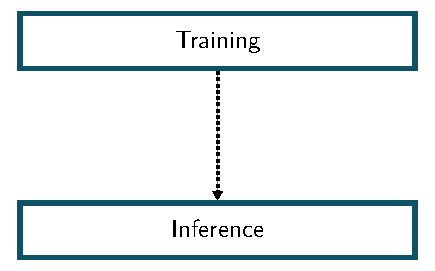
\includegraphics{ml_workflow_1.pdf}
		\subcaption{Traditional without inference optimization}\label{fig:ml-workflow-old}
	\end{minipage}%
	\begin{minipage}[b]{.5\textwidth}
		\centering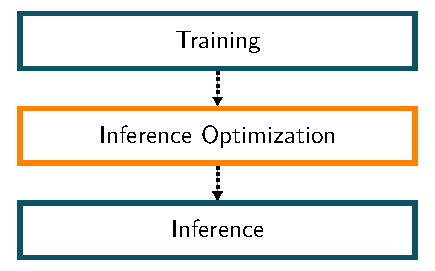
\includegraphics{ml_workflow_2.pdf}
		\subcaption{Improved with inference optimization}\label{fig:ml-workflow-new}
	\end{minipage}
	\caption[Traditional vs. optimized machine learning workflow]{Machine learning workflow}
	\label{fig:ml-workflow}
\end{figure}

The model determines what tensor operators are calculated, but it does not specify how they are calculated. Deliberately choosing the actual implementation offers great optimization potential. There is always a generic naïve implementation, which is the straightforward way of performing the calculation. However, it does not consider, e.g., memory sharing between threads or cache access patterns, which can have a significant adverse effect on performance~\cite{Hu.2017}. Techniques such as loop unrolling, reordering and tiling as well as multi-dimensional threading and tensor compute instructions can help leverage the accelerator's capabilities, but there is an abundance of combinations of settings for these techniques, the best of which is very much specific to the target device~\cite[p.~2]{Chen.2018b}. Finding the optimal such combination is the key aspect of tensor operator optimization.

Convolution operators are computationally very intensive and make up the majority of modern \glspl{cnn}, such as Inception\cite{Szegedy.2015} and ResNet\cite{He.2015}. Therefore, tensor operator optimization should focus on convolution over other types like pooling and fully-connected. It is not possible to optimize convolutions in general, but we need to optimize for every distinct parameter set that is present in the computation graph, i.e. combination of input shape, kernel shape, padding, and stride. This means that the effort increases with a higher variety of layer configurations.

\section{Manual Optimization}
Optimized implementations for tensor operators with a specific parameter set are provided by accelerator vendors in libraries like cuDNN for NVIDIA \glspl{gpu} and Intel Math Kernel Library for Intel CPUs. The vendors possess the hardware-specific knowledge to write good implementations by hand, but human expertise is required for this approach. While state-of-the-art, manual optimization has a number of inherent shortcomings:
\begin{itemize}
	\item slow support for new devices
	\item slow support for new graph-level optimizations
	\item no support for unconventional shapes
	\item vendor lock-in
\end{itemize}
These limitations hinder innovation, which is undesirable in a field so fast-evolving and relatively young as \gls{dl}. Researchers need to make a choice between avoiding devices, high-level optimizations and new network architectures that are not supported by those predefined operator libraries, and using unoptimized implementations~\cite[p.~1]{Chen.2018b}.

\section{Automated Optimization}
Automated tensor operator optimization, or \textit{autotuning}, overcomes these shortcomings by eliminating the need for human experts. Vendor-agnostic frameworks can discover good implementations regardless of hardware, model or graph optimizations. This enables innovation by fostering experimentation with novel or unconventional layers and high-level transformations that are not supported by manual libraries. Autotuning can achieve the same, in some cases even better inference performance than state-of-the-art vendor-provided operator libraries. Compared to these libraries, autotuning delivers speedups of 0.98× to 3.5× on CPU~\cite[p.~9]{Liu.2019} and 1.6× to 3.8× on server-class \glspl{gpu}~\cite[p.~10]{Chen.2018b} for commonly used \glspl{cnn}. Even a slightly worse performance is impressive considering that no domain-specific expert knowledge has been applied but only a few hours of autotuning.

Autotuning works by exploring the space of possible implementations in an organized fashion. Functionally equivalent implementations can be generated by a \textit{schedule} which defines a series of parametrized transformations that can are applied to the naïve implementation. The \textit{search space} is defined by the set of permutations of parameter settings. The settings control, for example, loop unrolling factors, loop order, loop tiling sizes and thread numbers, and can usually be adjusted in steps of powers of 2~\cite[p.~5]{Chen.2018b}~\cite[p.~16]{Vasilache.2018}. One specific combination of settings, i.e. one element of the search space, is called \textit{configuration}. Defining the values a setting can take is done manually for each class of target devices, but the search is guided by an algorithm that proposes candidate configurations. This is necessary since the size of the search space makes the brute-force approach of trying all configurations infeasible. As an example, the search space size for a ResNet-18 on an NVIDIA \gls{gpu} exceeds 172 million possible configurations, any one of which could be the best. \Gls{ml}-based or genetic algorithms help with rapid convergence to a decent, or ideally the best configuration without need of exhausting the whole search space.

\begin{figure}
	\begin{minipage}[b]{.45\textwidth}
		\small
		\centering
		\begin{minipage}{\textwidth}
			\begin{center}
				$ C = A^{T}B $
			\end{center}
			\unskip
			\subcaption{Mathematical expression}\label{fig:expr-sched-example-1}
		\end{minipage}
		\begin{minipage}{\textwidth}
		\begin{center}
			\bigskip
			$ C = sum(A[k, y] * B[k, x], axis=k) $
		\end{center}
		\end{minipage}
		\subcaption{Tensor index expression}\label{fig:expr-sched-example-2}
	\end{minipage}%
	\hfill
	\scriptsize
	\begin{minipage}[b]{.5\textwidth}
		\centering
		\begin{pythoncode*}{linenos=false,frame=none}
for y in range(1024):
  for x in range(1024):
    C[y][x] = 0
    for k in range(1024):
      C[y][x] += A[k][y] * B[k][x]
		\end{pythoncode*}
		\unskip
		\subcaption{Naïve low-level code}\label{fig:expr-sched-example-3}
	\end{minipage}
	\begin{minipage}[b]{.4\textwidth}
		\centering
		\bigskip
		\begin{pythoncode*}{linenos=false,frame=none}
for yo in range(128):
  for xo in range(128):
    C[yo*8:yo*8+8][xo*8:xo*8+8] = 0
    for ko in range(128):
      for yi in range(8):
        for xi in range(8):
          for ki in range(8):
            C[yo*8+yi][xo*8+xi] +=
              A[ko*8+ki][yo*8+yi]
                * B[ko*8+ki][xo*8+xi]
		\end{pythoncode*}
		\unskip
		\subcaption{Tiled low-level code}\label{fig:expr-sched-example-4}
	\end{minipage}
	\hfill
	\begin{minipage}[b]{.6\textwidth}
		\centering
		\bigskip
		\begin{pythoncode*}{linenos=false,frame=none}
inp_buffer AL[8][8], BL[8][8]
acc_buffer CL[8][8]
for yo in range(128):
  for xo in range(128):
    vdla.fill_zero(CL)
    for ko in range(128):
      vdla.dma_copy2d(AL, A[ko*8:ko*8+8][yo*8:yo*8+8])
      vdla.dma_copy2d(BL, B[ko*8:ko*8+8][xo*8:xo*8+8])
      vdla.fused_gemm8x8_add(CL, AL, BL)
    vdla.dma_copy2d(C[yo*8:yo*8+8,xo*8:xo*8+8], CL)
		\end{pythoncode*}
		\unskip
		\subcaption{Low-level code with accelerator-specific instructions}\label{fig:expr-sched-example-5}
	\end{minipage}
	\caption[Expressions and low-level code for transposed matrix multiplication]{Expressions and low-level code for transposed matrix multiplication~\cite[p.~4]{Chen.2018b}}
	\label{fig:expr-sched-example}
\end{figure}

Figure \ref{fig:expr-sched-example} provides an example of how different configurations affect the generated low-level code. The operator functionality is some mathematical calculation, in our example a transposed matrix multiplication (\ref{fig:expr-sched-example-1}). Before autotuning, that functionality is specified in a tensor expression language, which describes how to compute each element of the output tensor from the input tensors using a concise notation (\ref{fig:expr-sched-example-2}). Note that this notation is implicit, meaning that it does not prescribe implementation details. The autotuning framework then makes the computation explicit by applying a schedule with specific parameters from the configuration to the operator's default code. The simple but naïve reference code can be used to check the correctness after complex transformation (\ref{fig:expr-sched-example-3}). The low-level code is an intermediate representation that allows transforms, e.g. tiling for memory locality (\ref{fig:expr-sched-example-4}) or accelerator-specific instructions for buffers and specialized tensor operators (\ref{fig:expr-sched-example-5}). The specific tiling factors and buffer sizes can be varied and are determined by the applied configuration~\cite[p.~4~ff.]{Chen.2018b}~\cite[p.~9~ff.]{Vasilache.2018}.

Since the low-level code is only an intermediate representation, target-specific code, e.g., LLVM assembly for CPU or a CUDA kernel for NVIDIA \glspl{gpu}, needs to be generated. The appropriate compiler then builds that code, possibly in parallel for multiple configurations in a batch, after which the implementation can be executed. For autotuning, the execution time is then profiled on the target device to evaluate the performance. The profiling result is then stored alongside the implementation and fed back to the algorithm that selects candidate configurations. This allows the algorithm to improve its proposals for the next batch~\cite[p.~15~f.]{Vasilache.2018}. The iterative autotuning process can be stopped when a sufficiently fast implementation has been found or no better one has been discovered in a long time. Then, the full computation graph can be used for inference with the best implementations that have been found in the autotuning process for all operators.

There are two frameworks that implement autotuning, which will be described now.

\subsection{TensorComprehensions}
\glsunset{tc}
\acrlong{tc}\footnote{\url{https://github.com/facebookresearch/TensorComprehensions}} (\acrshort{tc}) has been developed by Facebook's AI Research team and comprises three main components: a language to express tensor computations (similar to Figure \ref{fig:expr-sched-example-2}), an optimizing compiler to generate efficient \gls{gpu} code from expressions, and an autotuner that finds good implementations and stores them in a compilation cache. It uses a polyhedral compiler to reason about and manipulate the loop structures of an implementation~\cite[p.~3]{Vasilache.2018}. However, only tensor-operators are considered, the framework is designed to be independent of computation graphs~\cite[p.~4]{Vasilache.2018}.

Autotuning in \gls{tc} starts from configurations that worked well for similar expressions, and some predefined strategies. The autotuner determines the configuration parameters and admissible value ranges. Then, a genetic algorithm generates a batch of candidate configurations. The value for each configuration parameter is randomly selected from one of three parents that are selected probabilistically based on their fitness. Furthermore, there is a low probability of mutation, which means that a random value is assigned to some parameters. Configurations are then compiled in parallel and profiled on an available GPU. A fitness value inversely proportional to the execution time is assigned to the configuration and stored in the autotuning database. Then, the process starts anew by selecting the next candidates using the updated database. This is repeated for a set amount of time~\cite[p.~15~f.]{Vasilache.2018}.

\subsection{TVM}
TVM\footnote{\url{https://github.com/dmlc/tvm/}} started as a research project at the University of Washington but is now supported and used by a large open-source community and companies like Amazon and Facebook. Unlike \gls{tc}, which only represents and optimizes tensor operators, TVM is an end-to-end \gls{dl} compiler stack. It can import whole models from a frontend framework and build minimal, optimized modules that can be deployed to backends like CPUs, \glspl{gpu} or FPGAs. Figure \ref{fig:tvm-stack} shows how the layers of the stack provide different levels of abstraction.

\begin{figure}
	\centering
	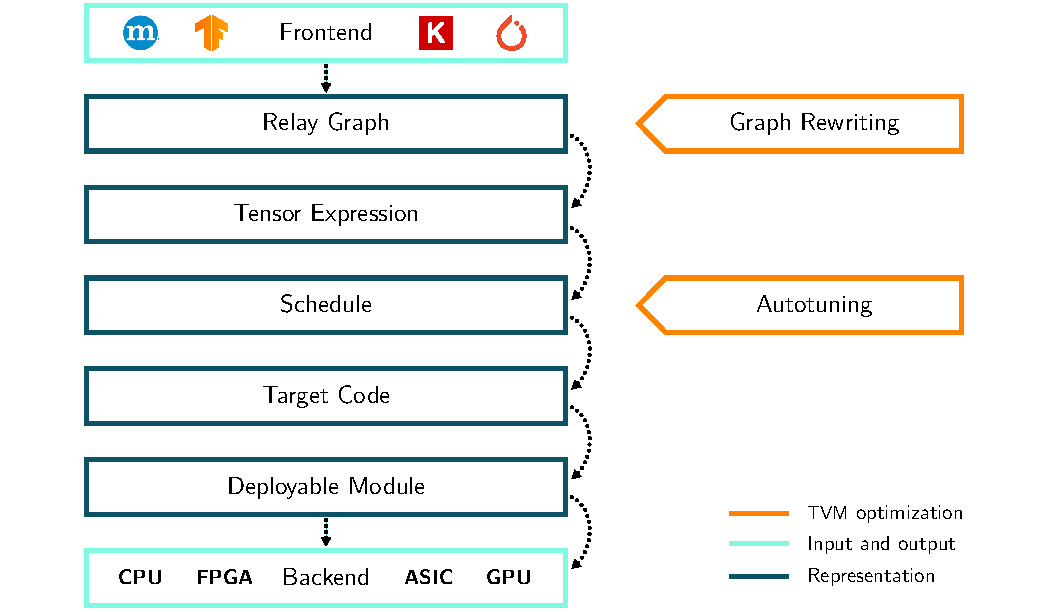
\includegraphics[width=\textwidth]{tvm_stack.pdf}%
	\caption{Levels of abstractions in TVM flow}
	\label{fig:tvm-stack}
\end{figure}

The top layer in the TVM stack is Relay. Relay is an intermediate model representation that enhances traditional computation graphs with concepts of functional programming to form a more powerful language. Relay supports shape-dependent tensor types and automatic differentiation, which is essential for \gls{dl} training~\cite[p.~61]{Roesch.2018}.  Additionally, a runtime to execute Relay programs in various programming languages is provided and needs to be present whenever executing TVM-based models. Relay programs can be created programmatically or from a textual source code. More convenient for users, however, is the import from diverse frontends, including TensorFlow, Keras, PyTorch and MXNet, which enables the use and optimization of existing models. Graph-level optimization in TVM is pass-based, with each pass inspecting or rewriting the syntax tree of the Relay program in some way. Standard passes are provided and perform, for example, automatic differentiation, type inference, operator fusion or tensor layout transformations~\cite[p.~3]{Chen.2018b}. Beyond that, writing custom passes is facilitated by an extensible design.

Next in the stack is a tensor expression language, which has similar features as \gls{tc}'s. It allows user to describe computation rules that generate a tensor without specifying loop structures and other details. The rules are composed of primitive mathematical operations like addition and multiplication and are expressive enough to describe tensor, matrix and vector operations. TVM comes with tensor expressions for common computations used in \gls{dl} such as various activation functions, convolution, pooling, and matrix multiplication~\cite[p.~4~f.]{Chen.2018b}. The tensor expression language is used to describe the functionality of tensor operators from the model. In the usual TVM workflow, the required operators are extracted from the Relay graph and matched with existing tensor expressions, so there is no need to write them manually.

Implicit tensor expressions need to be mapped to explicit, backend-independent loq-level code. TVM, again, uses a pass-based design, which is different from \gls{tc}'s polyhedral approach. Basic transformations called schedule primitives are combined into schedules that are applied to the naïve straightforward implementation to, for example, change loop structures and thread binding. This design is based on the Halide language for image processing, which works with similar multi-dimensional data as \gls{dl}, but enhances it with more primitives to optimize accelerator performance. TVM leverages nested and cooperative parallelism to make effective use of \gls{gpu} memory structure by enabling data reuse across threads through shared memory regions. This is done in a special memory scoping pass. TVM also equips the low-level code with hardware-specific instructions through a tensorization pass which matches computations patterns with a corresponding intrinsic from the target (such as general matrix multiply), making it extensible for new hardware architectures. A latency hiding pass introduces explicit management of fine-grained synchronization for memory and computation instructions on specialized \gls{dl} accelerators~\cite[p.~5~f.]{Chen.2018b}. Default schedule templates are provided for every hardware type, but users can create their own templates to incorporate their knowledge of the backend.

Low-level code cannot be executed, but it can directly be converted to target-specific code and then compiled for the target device. Backend-specific code generators create the source files, which are then built by the respective compiler and packed into a module which contains the implementation of all tensor operators in the model. This module can be deployed along with a JSON description of the Relay graph and a parameter file containing the weights for all operations. The TVM runtime (\SIrange{300}{600}{\kilo\byte}) needs to be installed on the target system to execute the model. However, a full \gls{dl} framework is not required, making TVM modules very lightweight to integrate into applications.

While \glspl{tc}'s autotuner is guided by a genetic algorithm, TVM uses a \gls{ml}-based cost model to predict the performance of an implementation. Specifically, gradient boosted trees are used because of their advantage in training and prediction speed over neural network-based models. Since the model is queried frequently, the inference overhead must be smaller than the profiling it seeks to replace. While profiling can be in the order of seconds, the gradient boosted trees model performs prediction in \SI{0.67}{\milli\second} on average. Model training time also needs to be considered; the cost model is updated periodically as more configurations have been explored, which improves the accuracy for further predictions with more experimental trials. This learning-based approach is preferable to static, predefined cost models for every new hardware target, which is infeasible due to the increasing complexity of modern accelerators~\cite[p.~8~f.]{Chen.2018b}. Pure low-level code cannot be used as input for the cost model, we need to encode it into a vector space first. This encoding needs to be a transferable representation which is invariant between programs to make the cost model effective. Encoding works by extracting context features from each loop level, including memory access count, reuse ratio of each memory buffer and loop annotations such as \enquote{unroll} or \enquote{parallel}. Furthermore, context relation features enable generalization across different loop nest patterns~\cite[p.~4]{Chen.2018}.

\begin{figure}
	\centering
	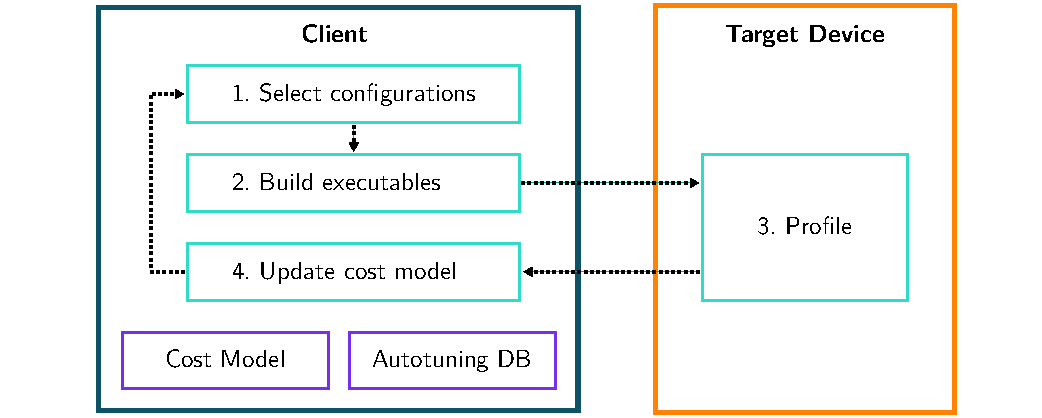
\includegraphics[width=\textwidth]{tvm_autotuning.pdf}%
	\caption{Iterative autotuning process in TVM}
	\label{fig:tvm-autotuning}
\end{figure}

Autotuning in TVM is an iterative process as seen in Figure \ref{fig:tvm-autotuning}. We call the component that executes the autotuning logic \textit{autotuning client}. Profiling the implementation requires execution on the actual target device. This can make autotuning a distributed process, if the client is another device. We call the execution of the autotuning process for one model a \textit{job}. However, autotuning is not performed for a whole model at once, but rather for a set of \textit{tasks} which correspond to autotunable tensor operators with a specific configuration (shapes, padding stride). These tasks need to be extracted from the model before starting the process for each of them. Autotuning consists of four stages that depend on each other, making it necessary to execute them in sequential order. Understanding the stages and their dependencies is key for enabling large-scale autotuning.

\begin{description}
	\item[Initialization] At the start of each task, profiling results from previous jobs are loaded from a global autotuning database, a file that contains data from all previous jobs along with information about the target and configuration. The loaded results are passed to the cost model for transfer learning. This yields good cost model from the beginning and improve in quality over time. Then the autotuning loop can be launched.
	\item[1. Select candidate configurations] At the start of each iteration, a batch of candidate configurations that have a promising performance is selected using the cost model. A simple strategy such as enumerating and running every configuration through the model, then selecting the top performers is impracticable with large search spaces. Rather, candidates are selected using parallel simulated annealing, which is a heuristic optimization algorithm that trades off finding an exact optimum for a much improved speed. Additionally, exploration is ensured by random selection of some configurations. If no training data exist yet, random candidates are picked.\footnote{In TVM's implementation, the selection of the next candidates is actually performed at the end of the iteration after updating the model, and the first stage just picks a batch from the already selected configurations. However, it is more logically simpler to think of the candidate selection using simulated annealing as part of the first stage. Furthermore, it is not wrong due to the iterative nature of autotuning.}
	\item[2. Build executables] The client combines the batch of configurations from the previous stage with the schedule template, then applies the schedule to the tensor expression for the operator of the current task. The resulting low-level code is then translated into backend-specific code and compiled. In case the target hardware is different from the client hardware, cross-compilation is necessary. The result is a tar file that contains everything that is necessary to run the executable, namely the compiled tensor operator itself and backend-specific code such as the CUDA driver library for NVIDIA \glspl{gpu}.
	\item[3. Profile on target device] Since the cost model's prediction of the implementation's performance are not completely reliable, the real performance needs to be evaluated on the target device. The tar files from the build stage are uploaded to the target device. Then the implementation is profiled by running the executable a number of times with random data. The measured execution times are averaged and returned to the client, which stores the results in the autotuning database for this job.
	. Parallel profiling on the same computation resource should be avoided to guarantee accurate results.
	\item[4. Update cost model] The cost model is updated with the measurements from the profiling stage to improve the proposed configurations in the next iteration. This is only done after a sufficient number of new profiling data has been collected, so this stage might be skipped in some iterations.
	\item[Finalization] After a certain number of trials, the loop is stopped. The best configuration that was discovered can now be used to build a faster implementation of the tensor operator that was optimized. Usually, the best configuration is also written into a separate database that contains only the best known configurations. The autotuning database for this job is merged with the global one. This concludes the autotuning process in TVM.
\end{description}

The target device is usually specialized for \gls{dl} workloads. Therefore, it is desirable to run the client on a machine that features a strong CPU to accelerate the compute-intensive build and profile stages. This distribution across multiple machines requires an \gls{rpc} infrastructure that makes it possible to profile on a different server. TVM's \gls{rpc} architecture (Figure \ref{fig:tvm-rpc}) comprises three components:
\begin{description}
	\item[Client] A client runs an autotuning job and and is responsible for selecting the candidate configurations, building the executables and updating the model with the profiling results. This means that the client contains both the cost model and the autotuning database. It also controls the profiling, but the actual execution is happening on servers.
	\item[Server] A server can receive and execute TVM modules, which basically makes it an RPC-enabled TVM runtime that runs on the target device. The interface on the client side does not change because TVM transparently handles remote execution like local execution. A server has a \textit{device key}, which is an arbitrary identifier for a certain device type, but usually is it based on the accelerator's name. Multiple servers can have the same device key if they run on identical target devices.
	\item[Tracker] A tracker keeps a list of servers to help clients discover unused servers for profiling. The tracker matches incoming requests from clients with free servers using a FIFO-based scheduling algorithm. Scheduling is implemented using a queue for servers and a heap for requests. Requests can have a priority.
\end{description}
TVM's \gls{rpc} is enabled by two distinct protocols. The control plane protocol is used for communication involving the tracker, namely server registration and requests from clients. The data plane protocol facilitates remote execution on a server and is initiated by clients.

\begin{figure}
	\centering
	
\includegraphics[width=\textwidth]{tvm_rpc.pdf}%
	\caption{TVM's RPC architecture}
	\label{fig:tvm-rpc}
\end{figure}

First, the tracker is started and listens on the first free port between 9190 and 9199. Then, one or multiple servers are started which bind to ports between 9091 and 9199. They register with the tracker by transmitting the device key, and the address and port which clients can use to connect. The tracker puts them in a queue, with separate queues for every device key. At this point, clients can request a server with a specific device key. The tracker matches the free server with that device key that registered first with the request that has the highest priority, then the one that was received first. If requests have the same priority, scheduling degrades to simple FIFO scheduling, and the request heap effectively becomes a queue. Once a client has acquired a server, it is marked as busy in the tracker and the client initiates a connection to the server to use its TVM runtime for profiling.

Since autotuning works in batches, usually not a single but multiple servers are requested to run profiling in parallel. This can speed up profiling if multiple target devices are available. For example, if a machine is equipped with 4 \glspl{gpu} of the target device type, 4 RPC servers can be launched on that machine, with each one being assigned to a different one of the \glspl{gpu}.

In this project, we use TVM instead of \gls{tc} because of the novel, machine learning-based approach, which promises better results than a genetic algorithm due to better guidance by the cost model. We are using the TVM version from June 11, 2019 (commit \href{https://github.com/dmlc/tvm/tree/8f219b9}{8f219b9}) for comparable results throughout the project. We made some modifications:
\begin{itemize}
	\item Add decomposed version of autotuner with separate methods for stages
	\item Add time measurement for autotuning stages
	\item Add loading of autotuning records from multiple files
	\item Fix Tensorflow import for models including PlaceholderWithDefault
\end{itemize}

	\chapter{Using TVM}
	For our end goal of enabling large-scale autotuning, we need to explore the current capabilities and limitations of TVM first, especially with regard to the execution of multiple autotuning jobs simultaneously. The modern \gls{dl} landscape is very diverse in terms of models and hardware, so to evaluate TVM in a diverse range of scenarios is crucial for gaining a proper understanding. To this end, we developed a framework that enables us to a large number of experiments rapidly.

\section{SimpleTVM}
Since using TVM follows a similar flow every time, we created SimpleTVM which exposes the individual steps through a convenient interface. This makes it easy for researches who are new to TVM to get started. FSince a lot of the experiments include benchmarking, time measurements are taken for most steps and automatically saved in a \textit{benchmarking context}. The flow of SimpleTVM has some dependencies, which are enforced. For example, a model needs to be imported before building. The interface including possible flows is depicted in Figure \ref{fig:simpletvm-interface}. The methods that are exposes are now regarded closer.

\begin{figure}
	\centering
	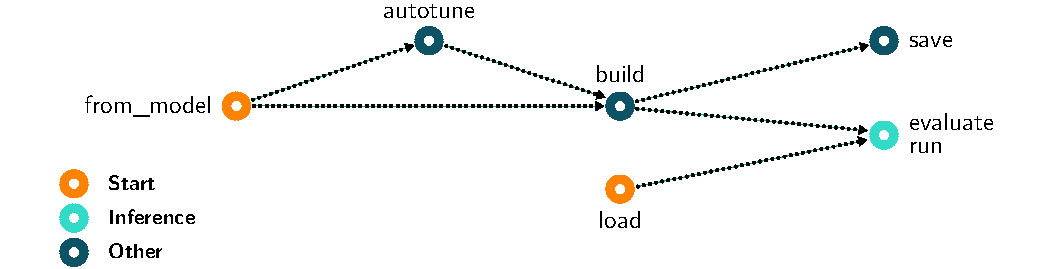
\includegraphics[width=\textwidth]{simpletvm_interface.pdf}%
	\caption{Interface and flow of SimpleTVM}
	\label{fig:simpletvm-interface}
\end{figure}

\begin{description}
	\item[\pythoninline/from_model/] Loading the Relay representation for the model is the beginning of a TVM flow. To that end, TVM supports the import from various frontends. Before the import of the model, however, it needs to be loaded and prepared for import. How exactly this is done differs even inside the same framework. SimpleTVM provides a unified import interface for TVM testing models, TensorFlow saved models (.pb files) and TensorFlow hub models. \pythoninline/from_model/ can easily be extended to support more frontends.
	\item[\pythoninline/autotune/] Once a model has been imported, autotuning can be run for each of the tensor operators. This step is optional, since TVM falls back to a default implementation if no records for that tensor operator exist in the autotuning database. Since this step is rather complex, there is a plethora of configuration options, the most important of which are exposed in \pythoninline/autotune/'s interface. SimpleTVM is designed to get new users started quickly so there are default values, but more experienced users can adjust the values according to their circumstances.
	\item[\pythoninline/build/] Before a TVM model can be executed, the target-specific executable needs to be build from the Relay model as described in the previous chapter. When building, SimpleTVM can either automatically use records from the global autotuning database, or the results from a specific autotuning job can be used.
	\item[\pythoninline/save/] After building, the library containing the operators can be saved along with the graph description and weights.
	\item[\pythoninline/load/] Beyond starting from an imported model, SimpleTVM can also load a previously saved TVM modules, which makes it possible to use a model that has been autotuned earlier. Saved modules can only be loaded if they have been built on the same device.
	\item[\pythoninline/run/] Inference can be run using this method. It accepts and returns a NumPy array. The input can, for example, be an image. However, loading the image and preparing it for inference, e.g., scaling and normalizing, needs to be done by the user.
	\item[\pythoninline/evaluate/] To profile the performance, \pythoninline/evaluate/ runs inference on random data multiple times, then averages the measured times. However, in contrast to the profiling stage of autotuning, not the performance of individual tensor operators but the whole model is measured.
\end{description}

An example of how SimpleTVM is typically used is presented in Listing \ref{lst:simpletvm-flow}. First, the \pythoninline/BenchmarkingContext/ is created (Line 1), which stores information about the current run such as the run id (a 32-character alphanumeric identifier for this execution of SimpleTVM), target device, measured times, the loaded model and the target device key to send to the tracker. When using a CPU as target device, the CPU architecture should be specified so TVM can select the proper hardware-specific tensor instructions. The benchmarking context is passed to the \pythoninline/SimpleTVM/ object (Line 2). Here, the address of the RPC tracker can be specified for distributed autotuning. If the address is not specified, autotuning will create a local tracker and server to perform autotuning on the same device as the client. Next, a model is imported (Line 3). Since the name of the output layer and the size of the output vector differs, it needs to specified explicitly. SimpleTVM's concise, chained syntax is used to autotune, build, save and evaluate the model (Line 4). For the sake of brevity, default parameters are leveraged, but the user can customize the actual calls to TVM functions by providing more parameters. Finally, the benchmarking context is saved (Line 5). This enables analysis at a later point, e.g., to examine the autotuning process or the inference performance measured by the evaluation. Note that this step is distinct from the saving of the TVM module. At a later point and usually by another application, the saved module which is identified by the run id can be loaded back. Then it can be used run inference on any data.

\begin{listing}
\begin{pythoncode}
ctx = BenchmarkingContext('cpu', device_key='i7', cpu_arch='skylake')
tvm = SimpleTVM(ctx, rpc_tracker=('tracker', 9190))
tvm.from_model('mobilenet.pb', output_name='out', output_size=10)
tvm.autotune().build().save().evaluate()
ctx.save()

# Saved model can be used later to run inference
tvm.load('run_id')
prediction = tvm.run(data)
\end{pythoncode}
\unskip
\caption{Typical SimpleTVM flow for CPU including autotuning}
\label{lst:simpletvm-flow}
\end{listing}

Additionally to SimpleTVM, we developed an automated benchmarking script called \textit{superb}. superb is short for \enquote{super benchmark} because it allows testing of different configurations without human intervention, so it performs benchmarking on a higher level than SimpleTVM's mechanisms. The user can specify the values for all parameters that should be tested. superb enumerates all possible combinations, effectively determining the $n$-ary product set of all value lists, then executes SimpleTVM once with each configuration. Additionally, it sets up the required servers and the tracker. The results from all configurations are collected and can then be processed by another script. This script evaluates the resulting inference performances, aggregates some information and writes them into a file, enabling further analysis with other tools such as Jupyter notebooks.

All SimpleTVM-related files are stored in the \enquote{\textasciitilde /.tvm-benchmark} directory. This includes the autotuning databases of currently running jobs, the global autotuning database and a file containing only the best known configurations. There are subdirectories for each SimpleTVM run with a log file for debugging, the saved benchmarking context and the autotuning log file for this run, if applicable. In another subdirectory, the results of superb experiments are collected with a csv file containing the aggregate information like mean autotuning time and the mean execution time for each stage. Finally, all saved modules are saved in a directory named after their run id.

Since we want to test TVM on a variety of machines, we created Docker images to be able to easily deploy TVM with all dependencies on any server. The \gls{gpu} version also includes the CUDA libraries, and a helper script for using the images mounts some folders into the container and sets up the environment. The Docker images in conjunction with SimpleTVM and superb form the foundation for our experiments.

\section{Parameters}
Autotuning with TVM offers a plethora of configuration options that affect both the autotuning process itself and the result. Setting these parameters to adequate values for the given job and hardware requires knowledge of how TVM works, but in some cases it is a matter of trial and error. However, guidelines and descriptions of the most important parameters can help. All of the following parameters can be specified when using SimpleTVM
\begin{description}
	\item[Number of trials] This determines the number of configurations to try for each autotuning task. A higher number will generally result in a better inference performance since the search space can be explored more, but this results in an increased autotuning completion time. However, the result starts to converge to the optimum after about 500 iterations, so there is a limit to the inference performance that can be achieved. Especially with CPUs, that have a small search space compared to \glspl{gpu}, there might not even be more options to try. Practically, the optimal result can be expected with the number of trials set to 2000.
	\item[Profiling timeout] This determines the time after which the profiling for one configuration is killed if it runs too long. Since every tensor operator has a different computational intensity and performance varies across types of hardware, this timeout needs to be adjusted accordingly. A high profiling timeout will allow longer execution, which drives up total autotuning completion time and might not yield better results since long-running implementations are not good and can safely be killed. A low profiling timeout might also kill of good implementations. It should be noted that the optimal timeout does not depend on the actual execution time, since profiling runs the implementation multiple times and might even dynamically adjust the number of executions. In practice, a low timeout should be set first. If the log shows too many timeout errors, the timeout can be increased. 5 seconds seems to be a good value for \gls{gpu} target devices, while 20 seconds or more are appropriate for CPU autotuning.
	\item[Batch size] This determines how many configurations are selected and built in parallel for every autotuning iteration. This can speed up autotuning considerably, especially if a large number of CPU cores are available on the client to run many compiler processes in parallel. The number of cores is also the default value. For larges batches, the model is updated and queried less frequently, but in general there seems to be no detrimental effect of having a high batch size. It should be notes that this is not the same as the batch size of the model, which would change the shape of the tensor operators.
	\item[Transfer learning] This determines whether or not transfer learning is used between jobs. According to this setting, the data from the global autotuning database might be used to train the cost model at the start of each task. Between tasks, there is always transfer learning. Usually, transfer learning should be enabled for the most optimal inference performance results. However, we disable transfer learning for experiments to guarantee a fair comparison between earlier and later ones.
\end{description}


\section{Capabilities}
Using SimpleTVM and our knowledge about proper parameter settings as foundation, we evaluated how TVM performs in comparison to state-of-the-art manual tensor operator libraries. We use TensorFlow 1.14 as baseline since it is a popular framework for \gls{dl} applications. cuDNN is enabled for \gls{gpu}. Autotuning with TVM was executed with 2000 trials, so the numbers should represent the optimal implementation. For evaluation, we test a Mobilenet with a batch size of one on two mobile-grade CPUs (Intel Core i5-5300U and i5-7300U), a server-grade CPU (Intel Xeon E5-2650 v3) and a high-end \gls{gpu} (NVIDIA Tesla K80). The same two images were used as model input in all cases.

\begin{figure}[h]
	\centering
	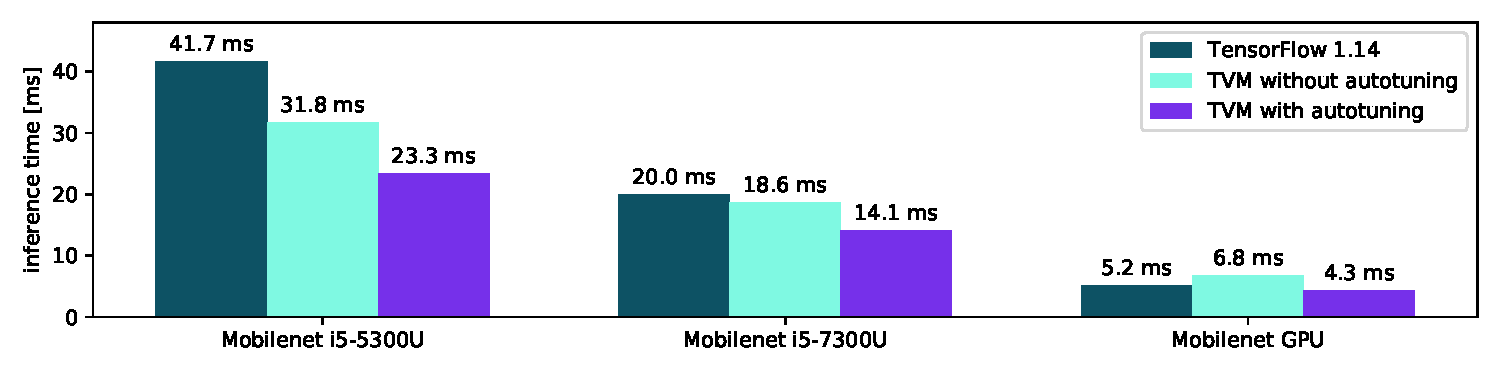
\includegraphics[width=\textwidth]{chart_inference_tf_vs_tvm}%
	\caption{Inference performance with TensorFlow and TVM}
	\label{fig:inf-tf-tvm}
\end{figure}

In all cases does TVM with autotuning show performance improvements over TensorFlow. Especially on CPU, inference speed improves by 44\% (\SI{18.4}{\milli\second}) for the i5-5300U and by 30\% (\SI{5.9}{\milli\second}) for the i5-7300U. But also for the \gls{gpu}, the autotuned version is 17\% (\SI{0.9}{\milli\second}) faster, albeit measurement inaccuracies are possible on this small time scale. Nonetheless, even a similar performance is impressive considering that no human expert knowledge was required and autotuning took less than \SI{6}{\hour} for CPU and less than \SI{12}{\hour} for \gls{gpu} (due to the much larger search space). Further results for a wider variety of devices and models, including recurrent neural networks, are provided in \cite{Chen.2018} and show similar improvements.\todo{Add analysis for Xeon}

TVM performs better than TensorFlow on CPU even without autotuning. Graph-level optimizations alone are enough to result in faster inference by 24\% (\SI{9.9}{\milli\second}) for the i5-5300U and by 7\% (\SI{1.4}{\milli\second}) for the i5-7300U. Since only a series of pre-defined transformation passes are applied to the Relay program, graph-level optimization is performed in a matter of seconds. However, non-autotuned TVM cannot keep up with TensorFlow on GPU, it is 31\% (\SI{1.6}{\milli\second}) slower.

These results show that TVM on par with manual optimization, at least for our limited evaluation scenarios. Furthermore, TVM is under active development and can be expected to show further performance improvements in the future.

\section{Limitations}
While the autotuning results are promising, we found that autotuning process suffers from some fundamental restrictions inherent to the current design which limit its efficiency. For all real measurements in this section, we evaluated autotuning of a ResNet-18 (12 convolutional layers, 1 fully-connected layer) with 2000 iterations per task on two machines with two Intel Xeon E5-2650 v3 CPUs and four Tesla K80 GPUs, one machine for client and target device each.

\subsection{Resource Utilization}
Since stages in autotuning depend on results of the previous stages (configurations are required for building, executables are necessary for profiling, time measurements are used to update the model), they need to be executed in sequence. Because profiling runs on the target device, the result is a lot of idle time on both the client and the target device. This sub-optimal resource\footnote{We define \textit{resource} as a machine that executes some stage in the autotuning process, e.g., the target device or the hardware that the client runs on.} utilization is exemplified in Figure \ref{fig:tvm-res-util}.

\begin{figure}
	\centering
	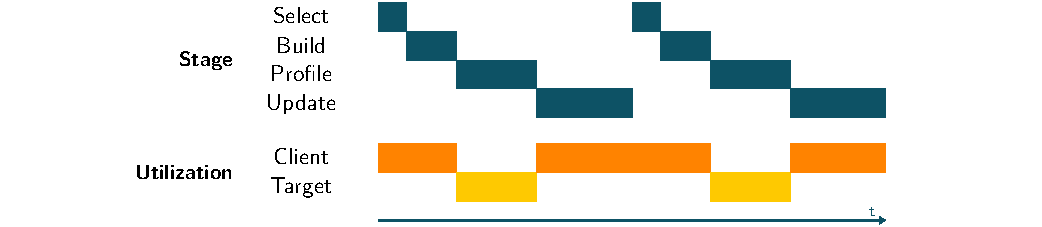
\includegraphics[width=\textwidth]{tvm_resource_utilization}%
	\caption{Resource utilization during autotuning}
	\label{fig:tvm-res-util}
\end{figure}

Measurements with our test setup showed that, for a total autotuning completion time of \SI{14.5}{\hour}, the client is idle for \SI{6.6}{\hour} (45\%) and the target device for \SI{7.9}{\hour} (55\%). Since computation resources, especially \gls{dl} accelerators, are rather costly, we want to minimize resource idle time. If existing resources are utilized better, it might not be necessary to acquire new hardware. If the individual occurences of idle time are long enough, it might be possible to use it for other computations in between. Indeed, the mean execution time for each stage is as follows: \SI{8.3}{\second} for building, \SI{39.5}{\second} for profiling, and \SI{44.0}{\second} for updating the model and selecting the next batch. This is long enough to reasonably assume that resource utilization can be improved by sharing the device. However, interference must be prevented.

\subsection{Scalability}
In preparation for enabling autotuning on a larger-scale, we need to examine the scalability of the current design. Scalability in this section refers to the ability to run an arbitrary number of autotuning jobs at the same time without sacrificing efficiency and result quality. We define objectives, that a scalable solution should satisfy:
\begin{enumerate}
	\item High inference performance, since it is the ultimate goal of autotuning
	\item Low amount of required hardware, since additional devices are costly
	\item Low autotuning time, since autotuning takes long
\end{enumerate}
These objectives are listed in order of priority. Good inference performance is the primary objective. It obviates the need to buy new hardware. Furthermore, there usually is a large amount of inferences which makes a longer autotuning time negligible over time. Rapid autotuning is nonetheless desirable.

We compare two setups for scaling that are possible using only the components that TVM comes with by default, schematically depicted in Figure \ref{fig:tvm-scaling-setups}. For the sake of simplicity, we only show depict two jobs, but this generalizes to any higher number. The evaluation of both setups with regard to the previously defined objectives is summarized in Table \ref{tab:tvm-scaling-setups}.

\begin{figure}
	\begin{minipage}[b]{.45\textwidth}
		\centering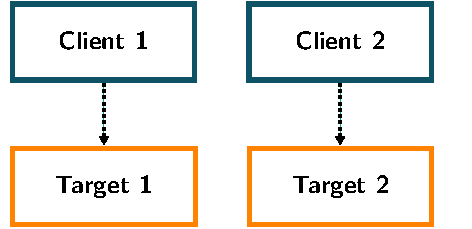
\includegraphics{scaling_setup_1}
		\subcaption{Dedicated resources}\label{fig:tvm-scaling-setups-1}
	\end{minipage}%
	\hspace{2em}
	\begin{minipage}[b]{.45\textwidth}
		\centering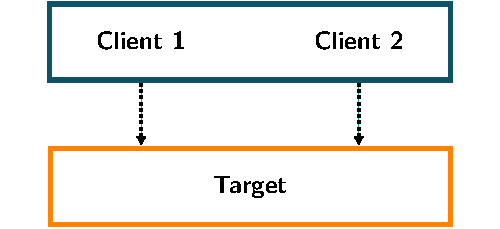
\includegraphics{scaling_setup_2}
		\subcaption{Shared resources}\label{fig:tvm-scaling-setups-2}
	\end{minipage}
	\caption{Setups for scaling autotuning}
	\label{fig:tvm-scaling-setups}
\end{figure}

\begin{description}
	\item[Dedicated resources] In the first setup (Figure \ref{fig:tvm-scaling-setups-1}), each job is run on its own set of resources. This means they are completely independent and do not affect each other. Both the resulting inference performance and the autotuning time are as good as possible, since they are equal to single-job autotuning. However, additional resources need to be acquired for every new job, which is not an economically feasible approach on a larger scale. Adding resources on demand from a cloud computing platform such as Amazon EC2 or Azure VM might work for the client machine, but since the actual target device needs to be used for profiling, which is likely to not be available on those cloud platforms, this is not a satisfactory solution. Alternatively to having separate sets of machines, the same machiens could be used to run the jobs in sequence. This trades off the amount of hardware that is required for autotuning time. With a higher number of jobs, this will take too long.
	\item[Shared resources] In the second setup (Figure \ref{fig:tvm-scaling-setups-2}), all jobs run in parallel on the same resource. To share the target device, we launch one RPC server for each client per GPU in our test setup. Due to the resource sharing, only one set of machines is required, which is good in terms of cost. However, this is very probable to lead to interference, when multiple jobs execute a stage on the same resource simultaneously. Interference has a detrimental effects on both inference performance and autotuning time. Interference on the client will slow down compute-intensive stages like building or model updates (50\%--70\% CPU usage). Modern CPUs are able to parallelize using multiple cores, but because building and model training uses all cores, time-sharing between multiple processes needs to be employed by the kernel. Process idle times and context switching overhead increase the autotuning time considerably. Assigning dedicated CPU cores per job will also make the process slower due to decreased resources per job and will not work when scaling up. Even more critical is interference on the target device. This distorts the profiling results, so good implementations might seem to perform bad if another job profiles on the same target device in parallel. Deceiving measurements will also lead to an inaccurate cost model. Since good inference performance is the prime objective of large-scale autotuning, this setup is also not satisfactory.
\end{description}

\begin{table}
	\newcommand\good[1]{\textcolor{hpe-green}{#1}}
	\newcommand\bad[1]{\textcolor{hpe-orange}{#1}}
	\newcommand\heading[1]{\textcolor{white}{\textbf{#1}}}
	\renewcommand{\arraystretch}{1.2}
	\sffamily
	\centering
	\begin{tabular}{l l l l}
	\rowcolor{black} \heading{Setup} & \heading{Hardware required} & \heading{Inference performance} & \heading{Autotuning time} \vspace{2pt} \\
	\textbf{Dedicated resources} & \bad{2x} & \good{High} & \good{Low} \\
	\textbf{Shared resources} & \good{1x} & \bad{Low} & \bad{High} \\
	\textbf{Optimum} & \good{1x} & \good{Low} & \good{Low} \\
	\end{tabular}
	\caption{Evaluation of setups regarding scalability objectives}
	\label{tab:tvm-scaling-setups}
\end{table}

Both setups do not meet all objectives we set for large-scale autotuning. Especially when scaling up to more parallel jobs, efficiency deteriorates significantly. We can conclude that the current implementation and architecture of autotuning in TVM does not scale well.

Having regarded possible scaling approaches and the reasons for their benefits and shortcomings, we can formulate two features for an optimal solution to satisfy the objectives:
\begin{itemize}
	\item Resources must be shared and utilized fully before adding new servers to minimize the required hardware for cost saving
	\item Interference must be prevented to guarantee a high inference performance and low autotuning time
\end{itemize}

\subsection{Similar Problems}
Our literature review was not successful in finding a solution to scale up autotuning. However, we can generalize the problem statement; we are looking for a solution to share available resources optimally between multiple tasks that are partially idle due to some dependency. From this point of view, we find two papers solving a similar problem.

\cite{Ma.2005} increases parallelism of a hierarchy of tasks and subtasks on multiprocessor platforms. Subtasks have control and data dependencies, but tasks are independent of each other. They employ a mix of exact and heuristic scheduling algorithms at design-time. Their scheduler interleaves sub-tasks of different tasks while respecting the dependencies between the subtasks of a single task. The result is a 37\% shorter execution time with increased resource utilization. The hierarchical structure of tasks and subtasks is similar to jobs and stages in autotuning.

\cite{Awatramani.2013} enable sharing of \gls{gpu} cores by multiple kernels. In current \gls{gpu} architectures, concurrently launched kernels use separate cores. However, interleaving of code from multiple kernels on the same core allows them to minimize core idle time introduced by memory latency. They increase the throughput of benchmarking applications by 7\%.

\cite{Ma.2005} and \cite{Awatramani.2013} improve parallelism for multiprocessing units while we want to improve parallelism for distributed machines. Nonetheless is the interleaving approach relevant.
	\chapter{Autotuning Scheduler}
	Interleaving of the stages of multiple jobs is our key concept for enabling large-scale autotuning. \cite{Ma.2005} uses a design-time scheduler to create a program with good concurrency. We need to dynamically schedule incoming jobs, so the schedule cannot be predetermined. We need an additional component in the autotuning architecture that orchestrates running jobs. In this chapter, we describe the design and implementation of our central scheduler that controls stage execution.

\section{Design}
Our scheduler possesses the two features that have been determined to be imperative for optimal large-scale autotuning:
\begin{itemize}
	\item Computation resources are shared between jobs. This facilitates good resource utilization since the idle time of one job can be harnessed to execute another job. This is called \textit{interleaving} and saves hardware and costs as a result. However, stage dependencies of a single job must be maintained.
	\item Interference between jobs is prevented. This guarantees that inference performance and autotuning time are as good as possible. The scheduler needs to check if the resource that will be used by the next stage is free before execution. This might necessitate the postponing of stage executions if the stage is ready before the resource becomes free.
\end{itemize}
These two features not only make it match the optimal solution, but also do they solve the problem of bad resource utilization of single-job autotuning by leveraging that shortcoming.

\begin{figure}[h]
	\centering
	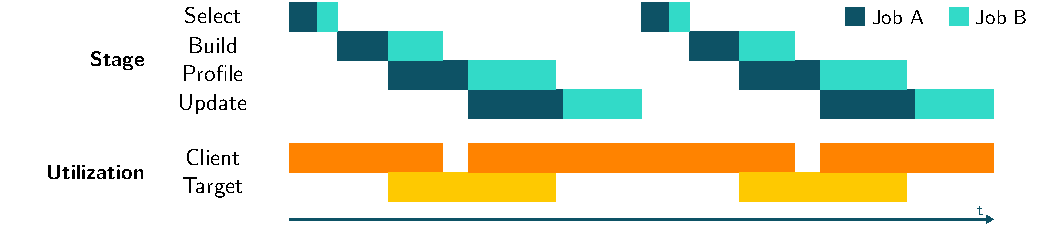
\includegraphics[width=\textwidth]{tvm_resource_utilization_interleaving}%
	\caption{Interleaving of multiple autotuning jobs}
	\label{fig:interleaving}
\end{figure}

Figure \ref{fig:interleaving} illustrates round-robin-based interleaving with an example of two jobs. Significant events are marked with numbers. Job A and Job B are started at the same time, but assume that the scheduler knows about A earlier. The first stage of A is executed, then the first stage of B. Once B finishes, the scheduler decides it is A's turn again and executes its second stage. Once A finishes the seconds stage, the client machine is free and B can execute the second stage. At the same time, A is ready to execute the third stage which will run on the target device. Since the target device is not in use, A can execute the profiling there in parallel to B's building since they use separate resources (\textbf{\textit{1}}). Building does not take as long as profiling, so A is ready to profile before B finishes its profiling stage. Therefore, A's third stage is postponed until the target device is free (\textbf{\textit{2}}). A's profiling and B's update model can, once again, execute simultaneously since they use distinct resources. After one iteration of all four stages, the process starts anew with the first stage (\textbf{\textit{3}}). This continues until both jobs are done. In a real scenario, new jobs might appear while other jobs are already running. The scheduler simply adds them to its list of jobs and includes them in the interleaving. Note how the resource utilization in Figure \ref{fig:interleaving} is much improved over the single-job autotuning in Figure \ref{fig:tvm-res-util} due to overlapping and sharing. Especially on the client device, utilization has almost been maximized since three of the four stages use the client.

\subsection{Autotuning Decomposition}
The default autotuning process is monolithic and can be regarded as a blackbox from the outside (Figure \ref{fig:autotuning-decomposition-before}). This means, the autotuning loop can be started, and it does not finish until the whole job is completed. Once a stage finishes, the next one is executed immediately. However, the scheduler needs to be able to control the execution of the individual stages because it needs to prevent interference by means of delayed execution. This necessitates the decomposition of the autotuning process into schedulable units, corresponding to the stages  (Figure \ref{fig:autotuning-decomposition-after}). The client does not execute any of the stages on its own. Rather, it provides an interface to execute schedulable units and waits for an external trigger to do so. The autotuning loop can now run in another component, such as the scheduler.

\begin{figure}
	\begin{minipage}[b]{.5\textwidth}
		\centering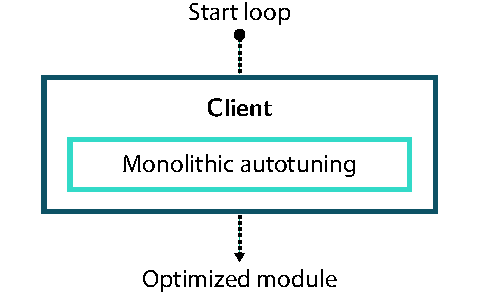
\includegraphics{autotuning_decomposition_before}
		\subcaption{Before decomposition}\label{fig:autotuning-decomposition-before}
	\end{minipage}%
	\begin{minipage}[b]{.5\textwidth}
		\centering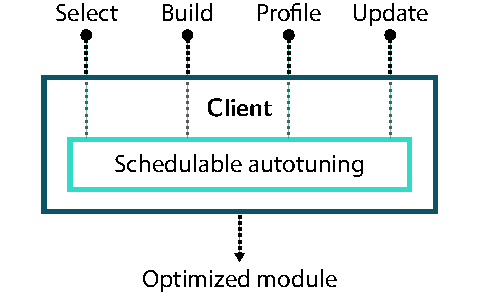
\includegraphics{autotuning_decomposition_after}
		\subcaption{After decomposition}\label{fig:autotuning-decomposition-after}
	\end{minipage}
	\caption{Client interface before and after decomposition}
	\label{fig:autotuning-decomposition}
\end{figure}

\subsection{Scheduling Algorithm}
To fulfill the task of interleaving while preventing interference, the scheduler needs to know four pieces of information for every job:
\begin{itemize}
	\item Whether the current stage is done; lets scheduler know if the job is ready for next stage
	\item Whether the whole job is done; lets scheduler know if the job needs to be considered in the future
	\item Which resource the current stage runs on; lets scheduler know which resources are free and which are in use
	\item Which resource the next stage will run on; lets scheduler postpone stage execution to prevent interference
\end{itemize}
We call this \textit{load-awareness}; being aware of the state of jobs and resources as well as their relationships. Theoretically, this allows the scheduler to work not only with TVM's autotuning but any process that can provide this information. Designing our scheduler to be agnostic of the underlying process also simplifies the algorithm since no state of this process, i.e. the progress or position in the loop, needs to be considered.

In case multiple jobs are ready to execute a stage, the scheduler needs to decide which one to run. The simplest approach is to use a round-robin algorithm, which iterates over the jobs in the order they were started and picks the first one that is ready. More sophisticated approaches might apply some logic to decide on a job which would maximize resource utilization but keep the average autotuning time low. However, we choose the round-robin algorithm for our first version. It is easy to implement and works reasonably well for an arbitrary number of jobs, which allows us to proof our concept.

We present two algorithms that perform interleaving. The greedy algorithm lets a job execute the next stage directly after the previous one finishes, provided the resource is free. This might preempt the resource from another job who is already waiting to execute a stage on it. On the other hand, the fair scheduler features a queue for every resource, so the first job to be ready to run a stage on a resource will be the first one to actually use it. Each job is controlled using an interface that provides the four pieces of information necessary for scheduling (\pythoninline/is_stage_done()/, \pythoninline/is_complete()/, \pythoninline/previous_resource/, \pythoninline/next_resource/). The scheduler keeps a list of jobs (\pythoninline/jobs/) in the order in which they were registered. With each call of \texttt{next()}, the subsequent job is returned, wrapping around after the end is reached.  Furthermore, it keeps a list of resources which can be marked as free or busy (\pythoninline/mark_as_free()/, \pythoninline/mark_as_busy()/).
\begin{description}
	\item[Greedy interleaving] The algorithm for greedy interleaved scheduling is presented in Listing \ref{lst:sched-algo-interleaving-greedy}. The algorithm is an infinite loop, with each iteration operating on one job (Line 1). First, the next job in the job list is retrieved (Line 2). If there is no job, the algorithm tries again until one is registered (Lines 3--4). If the job is still busy executing a stage, it is not considered further in this iteration (Line 6). If the stage has finished, the resource it used is marked as free (Line 7). If the stage was the last stage in the job, the job can be removed from the list of jobs (Line 8--9). Otherwise, the job is ready to continue. If the next stage's resource is free, that resource is marked as busy and the stage is executed immediately (Lines 11-13).
\begin{listing}[h]
\begin{pythoncode}
while True:
    job = jobs.next()
    if not job:
        continue

    if job.is_stage_done():
        mark_as_free(job.previous_resource)
        if job.is_complete():
            jobs.remove(job)
            continue
        if is_free(job.next_resource):
           mark_as_busy(job.next_resource)
           job.next_stage.execute()
\end{pythoncode}
\unskip
\caption{Greedy interleaved scheduling pseudocode}
\label{lst:sched-algo-interleaving-greedy}
\end{listing}
	\item[Fair interleaving] The algorithm for fair interleaved scheduling is presented in Listing \ref{lst:sched-algo-interleaving-fair}. Each resource has a queue which contains stages that are ready and will use that resource (Line 1). The algorithm is an infinite loop (Line 2), with each iteration consisting of two phases: scheduling and execution. In the first phase, the scheduler checks for each job if the current stage is done (Lines 4--5). Busy jobs are not regarded further. If the stage is done, the resource that was used is marked as free (Line 6). If the job is complete, it can be removed from the list of jobs (Line 7--8). Otherwise, the job is ready to continue and the next stage is added to the queue of the resource that it will run on (Line 9--10). The iteration over all jobs in order is what effectively makes this round-robin scheduling. In the second phase, the scheduler iterates over each resource and the corresponding queue (Line 12). If the resource is free and there are pending stages for that resource, the first stage in the queue is dequeued and executed (Lines 13--15). The respective resource needs to be marked as busy (Line 16).
\begin{listing}[h]
\begin{pythoncode}
queues = {r: [] for r in resources}
while True:
 # Phase 1: Round-robin scheduling
 for job in jobs:
     if job.is_stage_done():
         mark_as_free(job.previous_resource)
         if job.is_complete():
             jobs.remove(job)
         elif not job.next_stage in queues[job.next_resource]:
             queues[job.next_resource].enqueue(job.next_stage)
 # Phase 2: Execution
 for resource, queue in queues:
     if is_free(resource) and len(queue) > 0:
         stage = queue.dequeue()
         stage.execute()
         mark_as_busy(resource)
\end{pythoncode}
\unskip
\caption{Fair interleaved scheduling pseudocode}
\label{lst:sched-algo-interleaving-fair}
\end{listing}
\end{description}

Additionally to interleaving, our scheduler supports two other strategies for executing multiple jobs, which will be used in the evaluation for comparison.

Sequential scheduling (Listing \ref{lst:sched-algo-sequential}) works similar to single-job autotuning without a scheduler. Jobs do not run in parallel, but the next job is only started when the previous one finishes. This renders consideration of resource free/busy state unnecessary, and stages do not need to be postponed. However, since it is controlled by the scheduler, we can calculate the overhead introduced by adding a scheduler component, e.g., due to communication between scheduler and client or scheduling itself.

\begin{listing}[t]
\begin{pythoncode}
while True:
    job = jobs.next()
    if not job:
        continue

    while not job.is_complete():
        if job.is_stage_done():
            job.next_stage.execute()
    jobs.remove(job)
\end{pythoncode}
\unskip
\caption{Sequential scheduling pseudocode}
\label{lst:sched-algo-sequential}
\end{listing}

Synchronous scheduling (Listing \ref{lst:sched-algo-synchronous}) forces parallel execution of the same stage of multiple jobs on the same resource, making it the exact opposite of interleaved scheduling. Postponed stage execution is applied here to guarantee full interference. We use this strategy to evaluate the worst case effect of interference. However, this only works for equal jobs, since there needs to be symmetry between stages of all jobs.

\begin{listing}[t]
\begin{pythoncode}
while True:
    current_jobs = jobs
    if len(current_jobs) < 2:
        continue

    while not any([j.is_complete() for j in current_jobs]):
        if all([j.is_stage_done() for j in current_jobs]):
            [j.next_stage.execute() for j in current_jobs]
    jobs.remove_all(current_jobs)
\end{pythoncode}
\unskip
\caption{Synchronous scheduling pseudocode}
\label{lst:sched-algo-synchronous}
\end{listing}

\subsection{Autotuning Process}
\begin{figure}[ht]
	\centering
	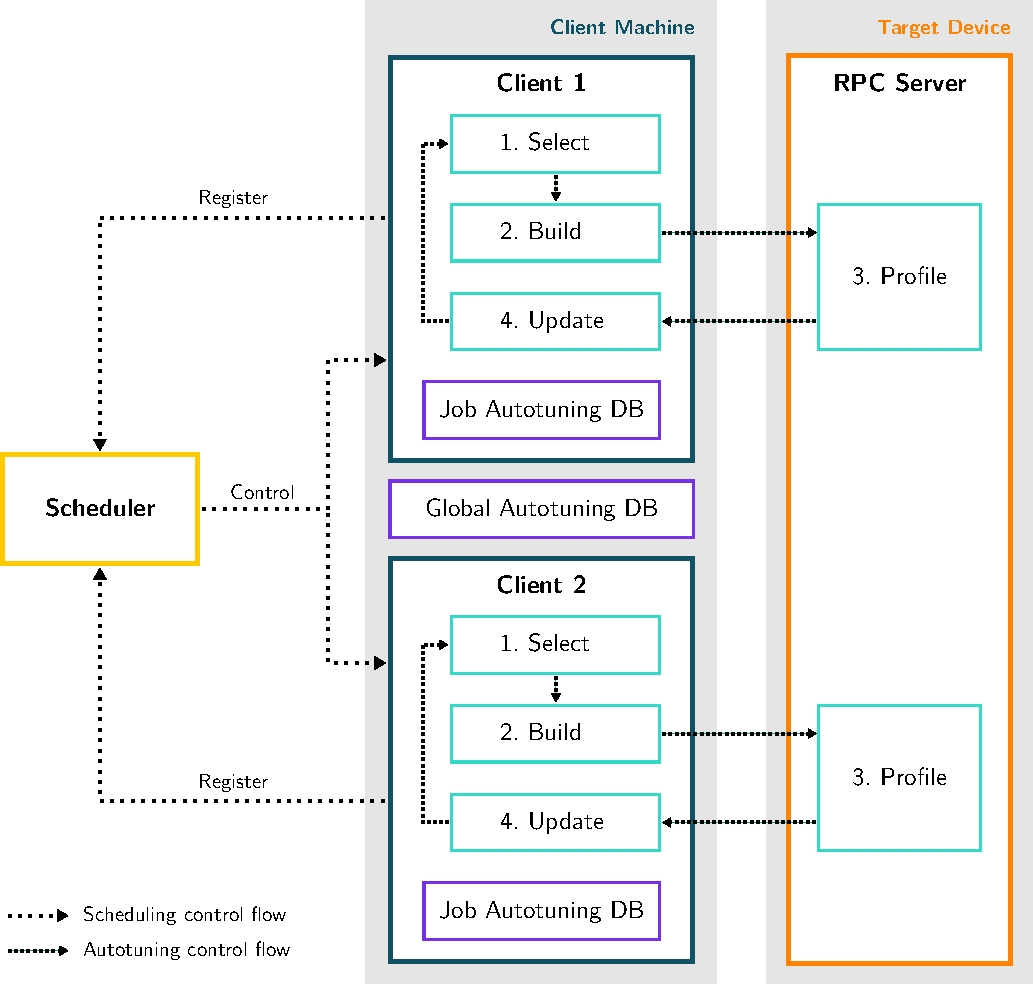
\includegraphics[width=\textwidth]{tvm_autotuning_with_scheduler.pdf}%
	\caption{Autotuning process with scheduler}
	\label{fig:tvm-autotuning-with-scheduler}
\end{figure}

Figure \ref{fig:tvm-autotuning-with-scheduler} shows the autotuning process with our scheduler (compare with scheduler-less, single-job autotuning in Figure \ref{fig:tvm-autotuning}). There are two discrete control flows at work. The per-job autotuning control flow is the same as before, spanning client and target machines. The scheduling control flow is on a higher level incorporating multiple jobs, and spans scheduler and clients. A new job needs to be made known to the scheduler first so it can consider the job in scheduling. One client is responsible for running exactly one job, registering that job with the scheduler when launching. The client is then ready to receive control commands to execute individual stages. The client exposes the interface which is required by the scheduling algorithm while calling the respective TVM methods internally. Clients can share target devices since the scheduler prevents interference of the profiling stages of multiple jobs on the same resource. The normal autotuning process is then executed, however not in one monolithic step, but stage for stage, enabled by the decomposition. Possibly there are some waiting times between stages introduces by postponing.

Scheduler and clients live in different processes, usually even separate containers or physical servers. While the autotuning control flow already exists in form of in-process method calls and \gls{rpc} for remote profiling, the scheduling control flow requires its own \gls{rpc} infrastructure to enable communication between the scheduler and the clients.

In multi-client scenarios, the cost model of each client is initialized by transfer learning from the global autotuning database on the client machine, which contains data from all jobs that have previously been executed on that machine. During autotuning, measurement results are written into a job-specific database which is merged back into the global database when the job is complete.

\section{Implementation}
Since TVM provides the API for autotuning in Python only, we use Python 3.6 for our implementation. It is intended as a proof of concept which we want to develop rapidly to see if the interleaving scheduler delivers the expected results. Therefore, we create an implementation that does not offer much flexibility or fault tolerance. However, it is sufficient to perform experiments in our test environment. The scheduler implementation is built on top of SimpleTVM for interfacing with TVM's autotuning.

For the beginning, only a single client machine is supported, but an arbitrary number of clients can run on it. Multiple target devices can be utilized for profiling, but the scheduler regards all target devices as a single resource. This coarse granularity is another decision to facilitate simple implementation.

\subsection{Components}
The implementation of our scheduler is distributed over multiple components. Same-machine components interact via in-process method calls, but \gls{rpc} is required for cross-machine calls. We created a simple HTTP-based \gls{rpc} protocol to support communication between scheduler and clients, with both scheduler and client acting as HTTP server and client. However, the protocol is very specific to the required interface and not general-purpose. If requests fail, they are retried three times with exponential backoff.

\begin{figure}[h]
	\centering
	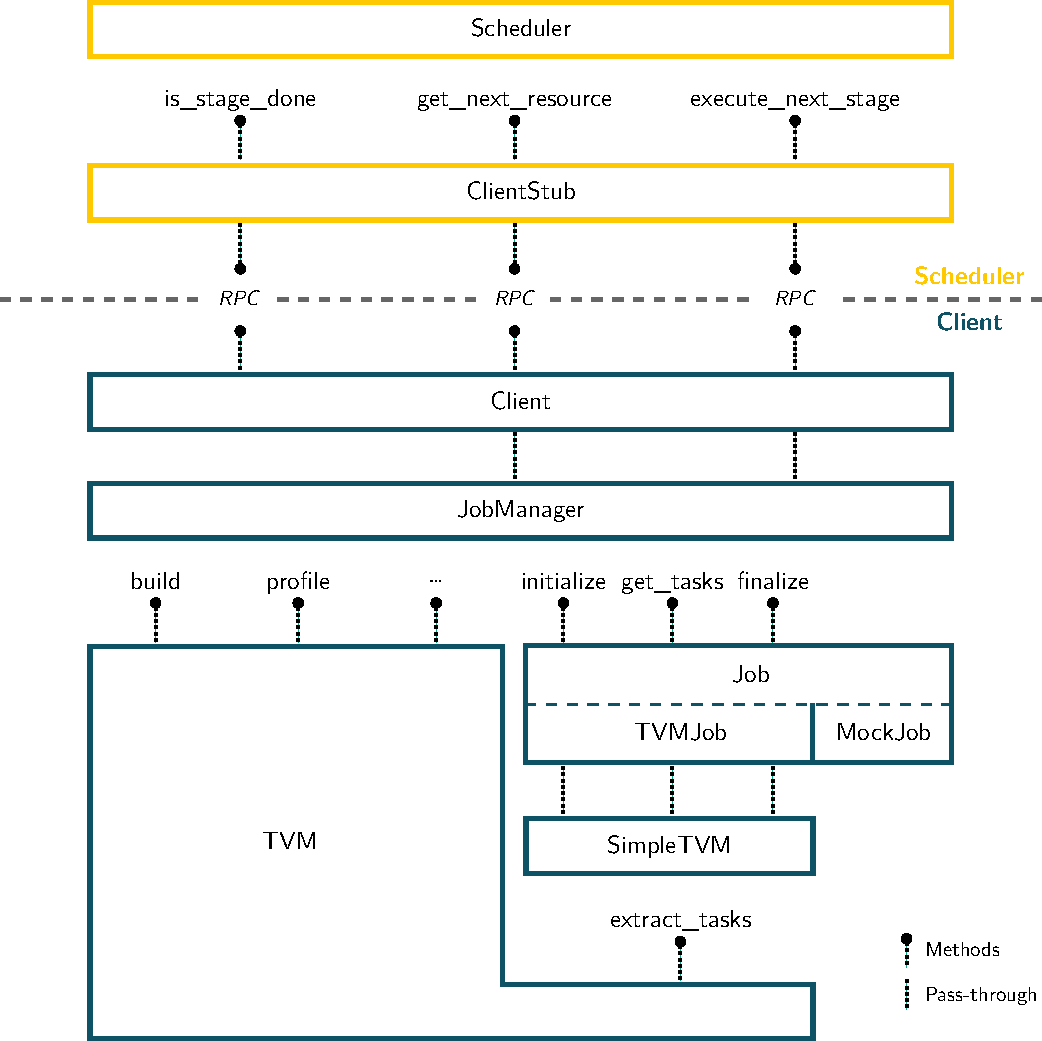
\includegraphics[width=\textwidth]{scheduler_layers}%
	\caption{Layers and components of scheduler implementation}
	\label{fig:scheduler-layers}
\end{figure}

The components act as layers of abstraction sitting on top of TVM to eventually hook into the actual autotuning process. Figure \ref{fig:scheduler-layers} shows the whole stack including method interfaces. We look closer at each component, from top to bottom.
\begin{description}
	\item[Scheduler] The \pythoninline/Scheduler/ implements the interleaved scheduling algorithms from Listings \ref{lst:sched-algo-interleaving-greedy} and  \ref{lst:sched-algo-interleaving-fair} as well as the sequential and synchronous strategies. The strategy can be specified when starting the scheduler. Instead of a list of jobs as in the algorithm, the scheduler actually keeps a list of the clients which run those jobs. The scheduler provides an \gls{rpc} interface for the client to register (not depicted in the figure) and will keep a reference to that client to enable controlling of its autotuning job. Additionally, some error handling is added to, e.g., remove clients if they become unreachable. Resource state is implemented in a resource--to--boolean dictionary, indicating if a given resource is free.
	\item[ClientStub] The \pythoninline/ClientStub/ does not perform any functionality on its own, rather it acts as an abstraction of the \pythoninline/Client/'s \gls{rpc} interface so the scheduler can call client methods as if they were an in-process object, allowing for a clean implementation of the scheduling algorithms. The \pythoninline/ClientStub/ passes through calls to the actual \pythoninline/Client/ but handles \gls{rpc} including serialization/deserialization of variables and error handling.
	\item[Client] The \pythoninline/Client/ provides the interface that is required by the scheduler to control jobs. It registers with the scheduler upon launch and exposes three methods via \gls{rpc}:
	\begin{itemize}
		\item \pythoninline/get_next_resource/ returns the resource that the next stage will run on, or \pythoninline/None/ if the job is complete, effectively combining two functionalities into one method. Furthermore, if the job is complete, the client shuts down after sending the \gls{rpc} response.
		\item \pythoninline/execute_next_stage/ calls the function for the next stage asynchronously and keeps a reference to the stage's thread in form of a future. If another stage is currently running, this methods fails.
		\item \pythoninline/is_stage_done/ returns a boolean, denoting if the stage that was previously executed using \pythoninline/execute_next_stage/ has finished. If no stage has been executed yet or the future indicates that the stage's thread has terminated,  \pythoninline/True/ is returned,  \pythoninline/False/ otherwise.
	\end{itemize}
	\item[JobManager] The \pythoninline/JobManager/ is responsible for negotiating between the simple resource- and stage-based interface required by the scheduler and the more complex interface of TVM's autotuning. This conversion from a stateless to a stateful interface requires that the \pythoninline/JobManager/ keep track of the current progress of the autotuning process, i.e. the position in the autotuning loop identified by task and stage. Effectively, it decides the order of stages in the loop, when the loop starts again, and when the loop terminates. This allows it to implement two methods: \pythoninline/get_next_resource/ is called directly by the client to get the resource that the next stage will run on, \pythoninline/get_next_stage/ returns a method containing the stage functionality which is executed by the client's \pythoninline/execute_next_stage/.\par
	The logic by which the next stage is decided in \pythoninline/get_next_stage/ is presented in Listing \ref{lst:stage-decision-algo}. \pythoninline/get_next_resource/ follows a similar logic but returns the resource instead of methods. The job's state is determined by flags indicating if the job has been initialized and finalized as well as the current task and stage in that task (Lines 1--2). If the job has not been initialized, the initialization method is returned and the \pythoninline/initialized/ flag is set (Lines 4--6). Then, the autotuning loop for the first task is started. With each call of \pythoninline/get_next_stage/, \pythoninline/current_stage/ is incremented and the respective stage's method is returned (Lines 8--22). The stage methods come from either the \pythoninline/Job/ or the decomposed TVM autotuning API. At the end of one loop iteration, which corresponds to one batch, the \pythoninline/current_stage/ is set to the first stage of the loop (Line 21). If the current batch was the last batch of the task (because either the search space has been exhausted or the specified number of trials has been reached), \pythoninline/current_task/ is incremented and \pythoninline/current_stage/ is reset to the task initialization so autotuning can commence for the next task (Lines 15--18). If all tasks have completed, the autotuning job is done (Line 7). Next comes the job finalization method (Lines 23--25), after which \pythoninline/None/ is always returned (Line 26).\par
\begin{listing}[h]
\begin{pythoncode}
initialized = finalized = False
current_task = current_stage = 0

if not initialized:
    initialized = True
    return initialize_job_fn
elif current_task < number_of_tasks:
    current_stage += 1
    if   current_stage == 1: return initialize_task_fn
    elif current_stage == 2: return select_batch_fn
    elif current_stage == 3: return build_fn
    elif current_stage == 4: return profile_fn
    elif current_stage == 5: return update_model_fn
    elif current_stage == 6:
        if last_batch:
            # Go to next task
            current_task += 1
            current_stage = 0
        else:
            # Go to select batch stage
            current_stage = 1
        return finish_batch_fn
elif not finalized:
    finalized = True
    return finalize_job_fn
else: return None
\end{pythoncode}
\unskip
\caption[{Pseudocode of JobManager's stage decision logic}]{Pseudocode of \pythoninline/JobManager/'s stage decision logic}
\label{lst:stage-decision-algo}
\end{listing}
	There is another version called \pythoninline/BundlingJobManager/ which exposes the same interface but instead of returning each stage individually, it bundles the stages for one resource into a single, larger stage. Thus, there are effectively only two stages, one for the client (select configurations, build, update model) and one for the target device (profiling), as opposed to \pythoninline/JobManager/ where each stage is individually schedulable. This might decrease resource idle time and speed up autotuning.
	\item[Job] The \pythoninline/Job/ is an abstract class which acts as interface specification for \pythoninline/TVMJob/ and \pythoninline/MockJob/. Jobs contain a collection of tasks as well as the initialization and finalization methods used by the \pythoninline/JobManager/.
	\item[TVMJob] The \pythoninline/TVMJob/ represents one autotuning job. It only passes calls through to \pythoninline/SimpleTVM/ which contains the implementations. The initialization method only stores a timestamp of the autotuning begin for measurement. The finalization method collects error and time statistics from the autotuning process and inserts them into the benchmarking context. Additionally, it merges the job-specific autotuning database with the global database. The collection of tasks is extracted using a method from TVM, but modified slightly by SimpleTVM.
	\item[MockJob] A \pythoninline/MockJob/ is a drop-in replacement for \pythoninline/TVMJob/, exposing the same interface but not running actual autotuning, which is a slow process. Rather, it simulates work by sleeping and prints to the console when stages are started and finished. This allows rapid debugging of the scheduler algorithms because no infrastructure like servers and the tracker need to be set up. The number of batches and tasks can be specified, as well as a time stretch factor to slow down or speed up the simulated work. The mock stages proportions are about the same as in real autotuning, e.g., profiling takes longer than building. It does not depend on any other components such as TVM.
\end{description}

\subsection{Usage}
Switching from scheduler-less default autotuning to scheduled autotuning is trivial if the former is already being used, as shown in Listing \ref{lst:simpletvm-flow-with-scheduler}. Creation of the \pythoninline/SimpleTVM/ object and import of the model is identical for both variants (Lines 1--2). Default autotuning is started by calling the appropriate method directly with the autotuning options such as number of trials or profiling timeout (Line 5). For scheduled autotuning, a \pythoninline/TVMJob/ needs to be created first (Line 8). A client for the job is then started with the host names of the client and scheduler machines as parameters (Line 9). After autotuning, the optimized module can be built, saved and evaluated as usual (compare Listing \ref{lst:simpletvm-flow}).
\begin{listing}[h]
\begin{pythoncode}
tvm = SimpleTVM(BenchmarkingContext('gpu'), rpc_tracker=('tracker', 9190))
tvm.from_model('resnet')

# Scheduler-less
tvm.autotune(options)

# Scheduled
job = TVMJob(tvm, options)
Client(job, client_host='client', scheduler_host='scheduler').start()
\end{pythoncode}
\unskip
\caption{Comparison of default and scheduled autotuning}
\label{lst:simpletvm-flow-with-scheduler}
\end{listing}

\subsection{Challenges}
For our very first prototype, we wanted all components to run in a single multi-threaded process, so we could evaluate our approach quickly without having to implement the \gls{rpc} protocol. However, Python does not support true multi-threading due to the global interpreter lock. This lock simplifies memory management for the interpreter but only one thread can execute code at a time because of it. Python's recommended replacement is launching other interpreter processes from within the code, however this requires serialization of objects for inter-process communication. Our nested class structures and passing around of methods that are created inside other methods caused problems with this serialization. That is why we had to implement \gls{rpc} before the actual scheduler to enable separate processes from the beginning.

Since multi-job autotuning with a scheduler requires setup of the infrastructure and is rather slow, we created the \pythoninline/MockJob/ class for improved debugging and testing of the scheduler functionality. This allows us to evaluate design choices in the scheduling algorithm much more rapidly. Moreover, the isolation from TVM narrows the room for errors which facilitates focusing on scheduler issues without being disrupted by problems caused by autotuning.

\section{Autotuning as a Service}
Setting up the multi-job autotuning infrastructure is cumbersome because a lot of components need to be configured and deployed, a lot of it imperatively in code. Additionally, provisioning of new client and target machines is not done automatically by the scheduler, which limits the scale at which autotuning can be performed. This motivates the need for an \gls{aaas} platform, which hides the complexity of building and maintaining the infrastructure and thus simplifies the application of autotuning, opening up the opportunities of autotuning for any developer of \gls{dl}-based software.

We imagine a solution that allows users to submit their trained model and a declarative specification, including information such as a target inference time to meet service-level agreements and the target device type such as specialized accelerators. The platform then automatically sets up the required machines and components, runs the autotuning process until the user's target inference time is achieved (or no further optimization is possible), then the optimized version is returned to the user. To this end, we propose a reference architecture. However, we do not implement the platform. \cite{Cho.2019} shows how the Kubernetes container management system could be harnessed for resource provisioning in an \gls{aaas} platform, with a prototype delivering promising results. Our architecture builds on top of such a system, however it does not prescribe any specific product.

\begin{figure}[h]
	\centering
	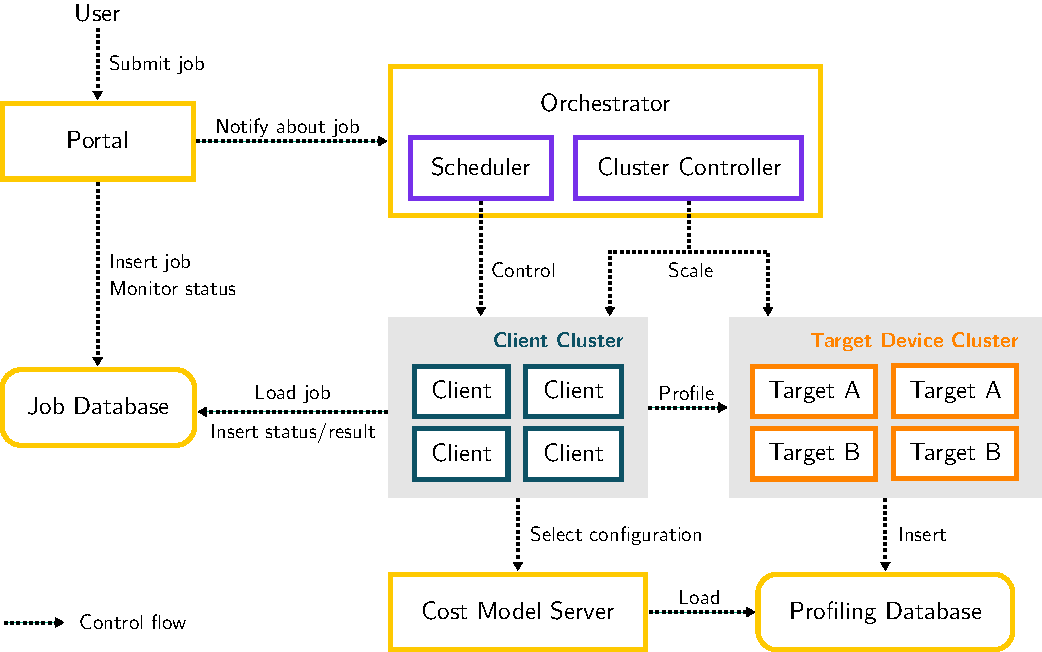
\includegraphics[width=\textwidth]{aaas_architecture}%
	\caption{Autotuning as a Service reference architecture}
	\label{fig:aaas-architecture}
\end{figure}

Figure \ref{fig:aaas-architecture} shows our proposed architecture. Users can submit their jobs including the model and specification through the portal. First the portal inserts that job information in the job database, after which it notifies the orchestrator about the new job. The orchestrator decides if the existing resources are sufficient, or if the client and target device cluster need to be scaled up, e.g., by booting new server instances on a cloud computing platform. The cluster controller, e.g., a Kubernetes Master, is responsible for executing the scaling. Then, the client is created on a client machine and the job is registered with the scheduler.
The scheduler now controls the autotuning jobs as described in the previous sections. However, the actual client functionality changes in the \gls{aaas} scenario. The cost model is extracted to a central server that all clients share, so neither a local cost model nor a job-specific autotuning database is necessary. The cost model server keeps a separate model for every target device. Furthermore, the client does not request profiling servers from a tracker, but the target devices are explicitly assigned per profiling stage by the scheduler. Profiling results are not returned to the client, but inserted into a global profiling database, which the cost model server uses to update the models periodically. Clients store their state in the job database as opposed to the JobManager object, which makes the clients stateless so they can resume the job in case of failure. This also allows the user to monitor autotuning progress through the portal. Once a job has completed, the resulting optimized TVM module is stored in the job database and the user can download it for deployment in his application.

Additionally, we make propose to increase autotuning speed. Firstly, before starting the autotuning, inference performance of a newly submitted model is checked with the existing best configurations. If the user's specifications are already met, no job needs to be launched. Secondly, jobs can be parallelized by splitting them into multiple jobs. Jobs consist of a set of tasks that are independent of each other. Moreover, the search space of each task can be divided to split one task into multiple. Leveraging task-level and search space-level splitting, autotuning can be accelerated if users request a higher number of resource be allocated to them. Furthermore, unused resources can be used better if the total platform load is low.

One limitation of \gls{aaas} over on-premise autotuning infrastructure is the set of supported target devices types. The platform can provide support for common accelerators, but if more exotic or novel hardware is desired, \gls{aaas} will fall short. One solution would be to support profiling on devices outside of the target device cluster. However, appropriate security measures would need to be taken.

In summary, the \gls{aaas} platform makes four important changes to the existing multi-job, scheduled autotuning architecture:
\begin{itemize}
	\item User-friendly portal instead of job specification in code
	\item Automatic resource provisioning/scaling instead of manual infrastructure setup
	\item Shared cost model between clients instead of job-local model
	\item External client state to recover from job failure instead of stateful clients
\end{itemize}
Instantiating such a platform is an important step towards making autotuning more accessible to enable more real-time \gls{dl} applications with little effort for developers.
	\chapter{Evaluation}
	To evaluate the impact of our scheduler, we compare the two approaches from Section \ref{sec:scalability} to our interleaving scheduler which aims to satisfy the \enquote{Optimum} solution. Additionally, we use the sequential scheduling algorithm as baseline while synchronous scheduling represents the worst case by forcing maximum interference. All scenarios are considered in terms of total autotuning completion time, time for the individual stages and the resulting inference performance.

Our evaluation environment consists of two identical machines with the following specifications:
\begin{itemize}
	\item 2x Intel Xeon E5-2650 v3, 10 cores, \SI{2.30}{\giga\hertz}
	\begin{itemize}
		\item Hyper-threading enabled
		\item AVX2 instruction set
	\end{itemize}
	\item \SI{128}{\giga\byte} main memory
	\item 4x Tesla K80 \glspl{gpu}, 4992 CUDA cores, \SI{24}{\giga\byte} memory
	\item Ubuntu 16.04.6 with Linux Kernel 4.4.0
	\item Python 3.6.8
\end{itemize}

Clients always run on the first machine, while profiling servers (TVM RPC servers) always run on the second machine whose \glspl{gpu} are used as target devices. Scheduler and tracker run on the first machine to decrease network latency. They do not interfere with autotuning since they are not computationally intensive.

The number of clients and profiling servers changes for every experiment, as shown in Table \ref{tab:tvm-evaluation-setups}. On \enquote{dedicated} servers, there is only one client. Two clients run on \enquote{shared} servers. Each profiling server of one client is assigned to a different GPU. Without interleaving, each client has its own set of four profiling servers, which might result in two servers if different clients being assigned to the same GPU. However, with interleaving, they can share the servers since they will never profile at the same time, eliminating competition.
\begin{table}
	\newcommand\heading[1]{\textcolor{white}{\textbf{#1}}}
	\renewcommand{\arraystretch}{1.2}
	\sffamily
	\centering
	\begin{tabularx}{\textwidth}{l l l l X}
	\rowcolor{black} \heading{Setup} & \heading{Server~~~~~} & \heading{Scheduler~~~~~~~~~~~~~} & \heading{Bundling~~~} & \heading{Profiling servers} \vspace{2pt} \\
	\textbf{A} & Dedicated & sequential & No & 4 \\
	\textbf{B} & Shared & sequential & No & 8 \\
	\textbf{C} & Shared & synchronous & No & 8 \\
	\textbf{D} & Shared & interleaved-greedy & No & 4 \\
	\textbf{E} & Shared & interleaved-fair & No & 4 \\
	\textbf{F} & Shared & interleaved-greedy & Yes & 4 \\
	\textbf{G} & Shared & interleaved-fair & Yes & 4 \\
	\end{tabularx}
	\caption{Evaluation setups}
	\label{tab:tvm-evaluation-setups}
\end{table}

All setups are controlled by the scheduler so each experiment is affected by the---albeit minimal---overhead of scheduling and \gls{rpc}. Two separate schedulers, one for each client, are used in B to achieve natural interference. \enquote{Bundling} indicates if stages of one resource are bundled into a single stage using the \pythoninline/BundlingJobManager/, or if each stage is individually scheduled.

Our test model is a ResNet-18, which consists of 12 convolution layers and one fully-connected layers, resulting in a job of 13 tasks. We autotune with 2000 trials per task and a profiling timeout of \SI{5}{\second}. Transfer learning from the global autotuning database is disabled so each experiment starts from the same, untrained cost model for a fair comparison. However, transfer learning is enabled between tasks. For time reasons, each experiment is only conducted once so the sample size is small.

A complete chart of all results can be found in Appendix \ref{sec:results}.

\section{Results}
First, we examine the impact of interference that was qualitatively described in Section \ref{sec:scalability}. We compare A, the optimum in terms of autotuning time and inference performance, with B and C (Figure \ref{fig:chart-interference-impact}). B lets jobs naturally interfere, while C forces maximum interference as worst case scenario. Interference is particularly noticeable for model updates since they are rather computationally intensive, which is why we show model update time in every figure.\\
The baseline completion time from A is \SI{14.5}{\hour}, \SI{6.1}{\hour} (42\%) of which are spent updating the model. Natural interference results in an increase in autotuning time by \SI{4.1}{\hour} (+28\%) while forced interference takes even \SI{5.0}{\hour} (+34\%) longer\footnote{For C, the time spent waiting for the other job to finish a stage introduced by the synchronous scheduling algorithm to force interference was subtracted from the total completion time since it would not occur naturally.}. This significant increase can be attributed to slower model updates, which witness a strong decline in performance. Compared with the baseline, the total time spent updating the model increases by \SI{3.8}{\hour} (+62\%) for B and by \SI{5.2}{\hour} (+85\%) for C. Build time only increases marginally, with profiling being slightly faster, possibly due to more timeouts. The baseline inference time is \SI{48.6}{\milli\second}. B is \SI{1.5}{\milli\second} slower, C is \SI{0.5}{\milli\second} slower. 

\begin{figure}[t]
	\begin{minipage}[b]{.6\textwidth}
		\centering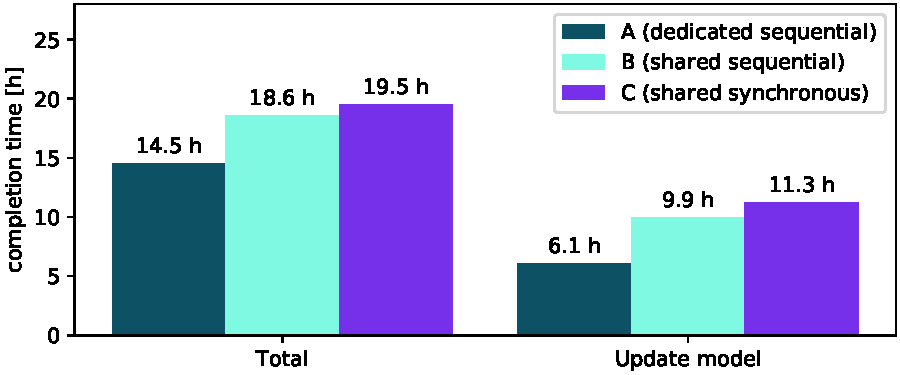
\includegraphics[width=\textwidth]{chart_interference_impact_completion}
		\subcaption{Completion time}\label{fig:chart-interference-impact-completion}
	\end{minipage}%
	\hfill
	\begin{minipage}[b]{.35\textwidth}
		\centering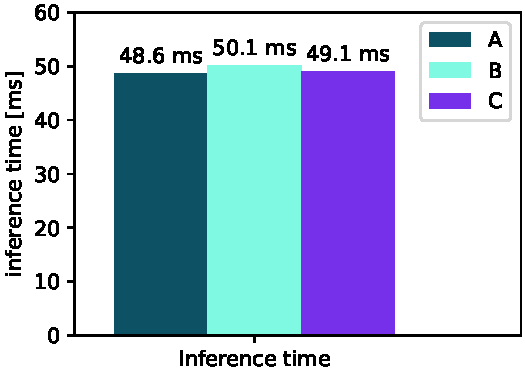
\includegraphics[width=\textwidth]{chart_interference_impact_inference}
		\subcaption{Inference performance}\label{fig:chart-interference-impact-inference}
	\end{minipage}
	\caption{Impact of interference}
	\label{fig:chart-interference-impact}
\end{figure}

We examine experiments D and E to evaluate the greedy and fair scheduler algorithm design, comparing them with A as baseline (Figure \ref{fig:chart-interleaving}). Using greedy interleaving, autotuning completes in \SI{20.4}{\hour}, \SI{5.9}{\hour} slower than A. While model update time stays about the same, \SI{5.5}{\hour} (27\%) of the total time is now spent waiting\footnote{Only stage execution times can be measured. Wait time and non-stage times (transfer learning, file operations) need to be derived. Non-stage times are about \SI{0.49}{\hour}, derived from A. Wait time for interleaving is calculated as follows: $t_{wait} = t_{total} - \sum_{i}t_{stage,i} - \SI{0.49}{\hour}$} for resources to become free to prevent interference. Fair interleaving is impacted even more by waiting, with total autotuning time increasing to \SI{24.1}{\hour}, \SI{9.6}{\hour} (+62\%) slower than A. Model update time remains about the same again, but wait time accumulates to \SI{8.9}{\hour} (37\% of total autotuning). Building and profiling time do not change for both. While the total completion time deteriorates, inference performance matches the baseline of \SI{48.6}{\milli\second} for both D and E.

\begin{figure}[t]
	\begin{minipage}[b]{.6\textwidth}
		\centering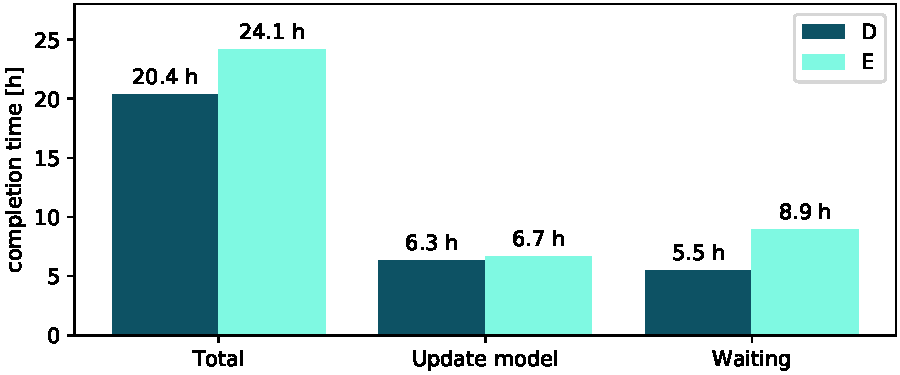
\includegraphics[width=\textwidth]{chart_interleaving_completion}
		\subcaption{Completion time}\label{fig:chart-interleaving-completion}
	\end{minipage}%
	\hfill
	\begin{minipage}[b]{.35\textwidth}
		\centering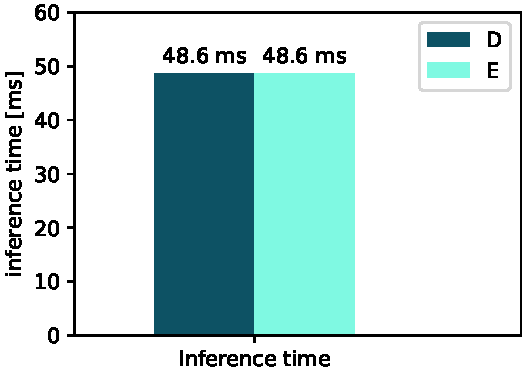
\includegraphics[width=\textwidth]{chart_interleaving_inference}
		\subcaption{Inference performance}\label{fig:chart-interleaving-inference}
	\end{minipage}
	\caption[Results of greedy versus fair interleaving]{Greedy versus fair interleaving}
	\label{fig:chart-interleaving}
\end{figure}

Finally, we examine the effect of employing stage bundling as opposed to individually scheduling them (Figure \ref{fig:chart-bundling}). The greedy algorithm is used in F, the fair algorithm is used in G. With bundling, greedy interleaving performs about the same as without bundling. On the other hand, fair interleaving completes \SI{2.4}{\hour} (-10\%) earlier than the individually scheduled version due to a total wait time that is \SI{2.7}{\hour} (-30\%) shorter. As before, model update time remains relatively similar. Inference time in F is \SI{0.4}{\milli\second} faster than in D, while G's is slower than E by \SI{0.3}{\milli\second}.

\begin{figure}[t]
	\begin{minipage}[b]{.6\textwidth}
		\centering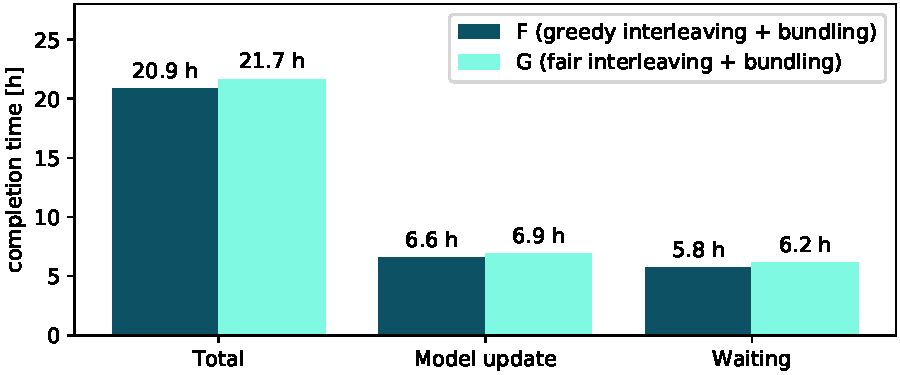
\includegraphics[width=\textwidth]{chart_bundling_completion}
		\subcaption{Completion time}\label{fig:chart-bundling-completion}
	\end{minipage}%
	\hfill
	\begin{minipage}[b]{.35\textwidth}
		\centering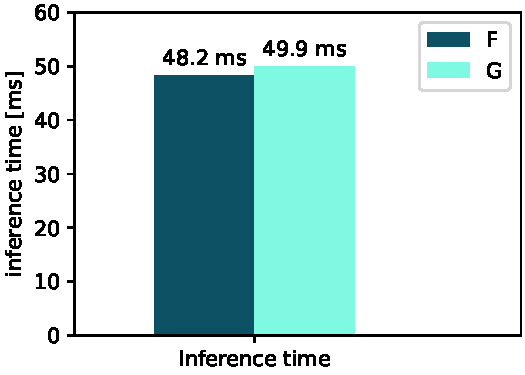
\includegraphics[width=\textwidth]{chart_bundling_inference}
		\subcaption{Inference performance}\label{fig:chart-bundling-inference}
	\end{minipage}
	\caption[Results of greedy versus fair interleaving with bundling]{Greedy versus fair interleaving with bundling}
	\label{fig:chart-bundling}
\end{figure}

\section{Discussion}
The objective of large-scale autotuning is to achieve the autotuning time and inference performance of running only a single job on each server, but with shared resources to keep the amount of required hardware at a minimum. Single-job autotuning is represented by Setup A, which is why we use it as baseline for comparisons with the other experiments. Because our evaluation is limited to a single machine type and model, more experiments are required for a general analysis.

In B and C we show the detrimental effects of interference on performance which motivated the creation of a scheduler. If it were not for this, resources could be shared and jobs could be run in parallel without control by a central entity. B and C behave relatively similar because even without explicit scheduling, both jobs run approximately synchronous since they autotune the same model. In real-world scenarios with diverse workloads, there might be a more drastic difference between B and C. The fact that C has faster inference than B is presumably caused by the probabilistic nature of configuration selection. The difference in inference performance of both to the baseline is relatively small due to the large number of trials which even out the impact of interference. However, even slightly worse inference speed has a large impact with an increasing number of inferences.

Note how interference is avoided with the scheduler in D--G, which manifests in stage times (particularly model updating) that are comparable to single-job autotuning as well as in a good inference performance. However, a significant amount of wait time is introduced which drives up total completion time. Greedy interleaving without bundling shows the shortest wait time in our experiments. Bundling does not show a big effect when comparing D and F because greedy interleaving naturally behaves like bundling. However, fair interleaving benefits much from bundling in our experiments, remedying the vast wait time.

Greedy interleaving works well in our experiments because both jobs are identical and the portion of time spent on the client machine versus time spent on the target device is roughly similar. As a result, wait time is reduced because, after an initial wait period, both jobs alternate nearly perfectly but mutually opposing between client and target. Despite these results, we believe that fair interleaving is the superior algorithm for scheduling heterogeneous jobs with varying complexity on a large scale, as would be the case with \gls{aaas}. Greedy interleaving would allow jobs to monopolize resources for an extended period of time, while fair interleaving allows for a finer control, especially if more resources are available. Bundling in conjunction with the fair algorithm is still an option to interleave homogeneous jobs on few resources, which would show the same effect as the greedy algorithm in our experiment.

Our scheduler is very rudimentary at this point, leaving much room for improvement. While the concept of interleaving seems promising, a more intelligent approach than fair round-robin could be employed to fill idle time optimally while keeping average wait time low. For example, a predictive scheduler could use knowledge from previous tasks to make a more educated decision that will maximize resource utilization. This would augment the notion of load-awareness with knowledge about the estimated stage execution time. Such a scheduler could then leverage the exact or heuristic interleaving algorithm from \cite{Ma.2005}. However, a more sophisticated algorithm might require finer control over the stages, which cannot be provided by the client's current resource/stage interface. Trading off a complex client but simple scheduler for a thin, stateless client and autotuning-aware scheduler by shifting responsibilities might become a necessity.

Furthermore, the scheduler needs to be enhanced with support for multiple resources of the same type. At this point, all target devices are regarded as a single, atomic resource. More granularity is essential for production-grade implementations in an \gls{aaas} platform. This would go hand in hand with eliminating the tracker and letting the scheduler assign target devices to clients. A trivial refinement is replacing the busy waiting for a stage to be done in the scheduler algorithm, resulting in an excess of redundant \gls{rpc} calls, by a push-based approach, where the client notifies the scheduler once a stage has completed.

We used our scheduler only for autotuning with TVM. However, other autotuning frameworks like \gls{tc} that have the same scaling issues might also profit from our solution. The \gls{aaas} platform might even provide support for a variety of autotuning frameworks.
	\chapter{Conclusion}
	Enabling large-scale autotuning is the foundation of any \gls{aaas} platform that uses our reference architecture. We demonstrated that our interleaving scheduler can leverage the fundamental weakness of resource idle time to make sharing of computation resources possible, which facilitates fast and economical autotuning while delivering good inference performance. This is a key step towards democratizing real-time \gls{dl} applications to power exciting innovations in a wide variety of fields.

Future efforts based on our work should focus on creating a more intelligent scheduler algorithm to improve the efficiency of multi-job autotuning. A resource provisioning algorithm will then complete the orchestrator component, paving the way for the development of a mature \gls{aaas} product.

	
	\clearpage
	
	%----------------------------------------------------------------------------
	% Appendix
	%----------------------------------------------------------------------------
	
	\cleardoublepage
	\printbibliography

	\printglossary[style=altlist]
	
	\clearpage
	\appendix
\end{document}